%%%%%%%%%%%%%%%%%%%% book.tex %%%%%%%%%%%%%%%%%%%%%%%%%%%%%
%
% Book template for lecture notes
%
%%%%%%%%%%%%%%%% Springer-Verlag %%%%%%%%%%%%%%%%%%%%%%%%%%


% RECOMMENDED %%%%%%%%%%%%%%%%%%%%%%%%%%%%%%%%%%%%%%%%%%%%%%%%%%%
\documentclass[graybox,envcountchap,sectrefs]{style/svmono}


%%%%%%%%%%%%%%%%% Book Formatting Comments:

%%%%%%%%%%%%%%%%%%%%%%%%%%%%%%%%%%%%% for Part

%%%%%%%%%%%%%%%%%%%%%% for chapter

%%%%%%%%%%%%%%%%%%%% for section








%%%%%% PACKAGES %%%%%%%
\usepackage{hyperref}
\hypersetup{
    colorlinks,
    citecolor=black,
    filecolor=black,
    linkcolor=black,
    urlcolor=black
}
\usepackage{amsmath} % Math display options
\usepackage{amssymb} % Math symbols
\usepackage{amsfonts} % Math fonts
\usepackage{amsthm}
\usepackage{mathtools} % General math tools
\usepackage{array} % Allows you to write arrays
\usepackage{empheq} % For boxing equations
\usepackage{mathabx}
\usepackage{mathrsfs}
\usepackage{nameref}

\usepackage{soul}
\usepackage[normalem]{ulem}

\usepackage{txfonts}
\usepackage{cancel}
\usepackage[toc, page]{appendix}
\usepackage{titletoc,tocloft}
\setlength{\cftchapindent}{1em}
\setlength{\cftsecindent}{2em}
\setlength{\cftsubsecindent}{3em}
\setlength{\cftsubsubsecindent}{4em}
\usepackage{titlesec}

\titleformat{\section}
  {\normalfont\fontsize{25}{15}\bfseries}{\thesection}{1em}{}
\titleformat{\section}
  {\normalfont\fontsize{20}{15}\bfseries}{\thesubsection}{1em}{}
\setcounter{secnumdepth}{1}  
  
  

\newcommand\numberthis{\refstepcounter{equation}\tag{\theequation}} % For equation labelling
\usepackage[framemethod=tikz]{mdframed}

\usepackage{tikz} % For drawing commutative diagrams
\usetikzlibrary{cd}
\usetikzlibrary{calc}
\tikzset{every picture/.style={line width=0.75pt}} %set default line width to 0.75p

\usepackage{datetime}
\usepackage[margin=1in]{geometry}
\setlength{\parskip}{1em}
\usepackage{graphicx}
\usepackage{float}
\usepackage{fancyhdr}
\setlength{\headheight}{15pt} 
\pagestyle{fancy}
\lhead[\leftmark]{}
\rhead[]{\leftmark}

\usepackage{enumitem}

\usepackage{url}
\allowdisplaybreaks

%%%%%% ENVIRONMENTS %%%
\definecolor{purp}{rgb}{0.29, 0, 0.51}
\definecolor{bloo}{rgb}{0, 0.13, 0.80}



%%\newtheoremstyle{note}% hnamei
%{3pt}% hSpace above
%{3pt}% hSpace belowi
%{}% hBody fonti
%{}% hIndent amounti
%{\itshape}% hTheorem head fonti
%{:}% hPunctuation after theorem headi
%{.5em}% hSpace after theorem headi
%{}% hTheorem head spec (can be left empty, meaning ‘normal’)i


%%%%%%%%%%%%% THEOREM STYLES

\newtheoremstyle{BigTheorem}
{20pt}
{20pt}
{\slshape}
{}
{\Large\color{purp}\bfseries}
{.}
{\newline}
{\thmname{#1}\thmnumber{ #2}\thmnote{ (#3)}}



\newtheoremstyle{TheoremClassic}
{15pt}
{15pt}
{\slshape}
{}
{\bfseries}
{.}
{.5em}
{}

\newtheoremstyle{Definitions}
{15pt}
{15pt}
{\slshape}
{}
{\bfseries}
{.}
{.5em}
{\thmname{#1}\thmnumber{ #2}\thmnote{ (#3)}}


\newtheoremstyle{Remarks}
{10pt}
{10pt}
{\upshape}
{}
{\bfseries}
{.}
{.5em}
{}

\newtheoremstyle{Examples}
{10pt}
{10pt}
{\upshape}
{}
{\bfseries}
{.}
{.5em}
{}


%%%%%%%%%%%%% THEOREM DEFINITIONS

\theoremstyle{BigTheorem}
\newtheorem{namthm}{Theorem}
\newtheorem{conj}[namthm]{Conjecture}

\theoremstyle{TheoremClassic}
\newtheorem{thm}{Theorem}[section]
\newtheorem*{thm*}{Theorem}
\newtheorem{lem}[thm]{Lemma}
\newtheorem{cor}[thm]{Corollary}
\newtheorem{prop}[thm]{Proposition}
\newtheorem{claim}[thm]{Claim}


\theoremstyle{Definitions}
\newtheorem{defn}{Definition}[section]
\newtheorem{axi}[defn]{Axiom}
\newtheorem{cust}[defn]{}
\newtheorem{cons}[defn]{Construction}
\newtheorem{props}[defn]{Properties}
\newtheorem{proc}[defn]{Process}
\newtheorem*{law}{Law}


\theoremstyle{Examples}
\newtheorem{eg}{Example}[section]
\newtheorem{noneg}[eg]{Non-Example}
\newtheorem{xca}[eg]{Exercise}


\theoremstyle{Remarks}
\newtheorem{rmk}{Remark}[section]
\newtheorem{qst}[rmk]{Question}
\newtheorem*{ans}{Answer}
\newtheorem{obs}[rmk]{Observation}
\newtheorem{rec}[rmk]{Recall}
\newtheorem{summ}[rmk]{Summary}
\newtheorem{nota}[rmk]{Notation}
\newtheorem{note}[rmk]{Note}



\renewcommand{\qedsymbol}{$\blacksquare$}


\numberwithin{equation}{section}

\newenvironment{qest}{
    \begin{center}
        \em
    }
    {
    \end{center}
    }

%%%%%% MACROS %%%%%%%%%
%% New Commands
\newcommand{\ip}[1]{\langle#1\rangle} %%% Inner product
\newcommand{\abs}[1]{\lvert#1\rvert} %%% Modulus
\newcommand\diag{\operatorname{diag}} %%% diag matrix
\newcommand\tr{\mbox{tr}\.} %%% trace
\newcommand\C{\mathbb C} %%% Complex numbers
\newcommand\R{\mathbb R} %%% Real numbers
\newcommand\Z{\mathbb Z} %%% Integers
\newcommand\Q{\mathbb Q} %%% Rationals
\newcommand\N{\mathbb N} %%% Naturals
\newcommand\F{\mathbb F} %%% An arbitrary field
\newcommand\ste{\operatorname{St}} %%% Steinberg Representation
\newcommand\GL{\mathbf{GL}} %%% General Linear group
\newcommand\SL{\mathbf{SL}} %%% Special linear group
\newcommand\gl{\mathfrak{gl}} %%% General linear algebra
\newcommand\G{\mathbf{G}} %%% connected reductive group
\newcommand\g{\mathfrak{g}} %%% Lie algebra of G
\newcommand\Hbf{\mathbf{H}} %%% Theta fixed points of G
\newcommand\X{\mathbf{X}} %%% Symmetric space X
\newcommand{\catname}[1]{\normalfont\textbf{#1}}
\newcommand{\Set}{\catname{Set}} %%% Category set
\newcommand{\Grp}{\catname{Grp}} %%% Category group
\newcommand{\Rmod}{\catname{R-Mod}} %%% Category r-modules
\newcommand{\Mon}{\catname{Mon}} %%% Category monoid
\newcommand{\Ring}{\catname{Ring}} %%% Category ring
\newcommand{\Topp}{\catname{Top}} %%% Category Topological spaces
\newcommand{\Vect}{\catname{Vect}_{k}} %%% category vector spaces'
\newcommand\Hom{\mathbf{Hom}} %%% Arrows

\newcommand{\map}[2]{\begin{array}{c} #1 \\ #2 \end{array}}

\newcommand{\Emph}[1]{\textbf{\ul{\emph{#1}}}}

\newcommand{\mapsfrom}{\mathrel{\reflectbox{\ensuremath{\mapsto}}}}


%% Math operators
\DeclareMathOperator{\ran}{Im} %%% image
\DeclareMathOperator{\aut}{Aut} %%% Automorphisms
\DeclareMathOperator{\spn}{span} %%% span
\DeclareMathOperator{\ann}{Ann} %%% annihilator
\DeclareMathOperator{\rank}{rank} %%% Rank
\DeclareMathOperator{\ch}{char} %%% characteristic
\DeclareMathOperator{\ev}{\bf{ev}} %%% evaluation
\DeclareMathOperator{\sgn}{sign} %%% sign
\DeclareMathOperator{\id}{Id} %%% identity
\DeclareMathOperator{\supp}{Supp} %%% support
\DeclareMathOperator{\inn}{Inn} %%% Inner aut
\DeclareMathOperator{\en}{End} %%% Endomorphisms
\DeclareMathOperator{\sym}{Sym} %%% Group of symmetries


%% Diagram Environments
\iffalse
\begin{center}
    \begin{tikzpicture}[baseline= (a).base]
        \node[scale=1] (a) at (0,0){
          \begin{tikzcd}
           
          \end{tikzcd}
        };
    \end{tikzpicture}
\end{center}
\fi




\newdateformat{monthdayyeardate}{%
    \monthname[\THEMONTH]~\THEDAY, \THEYEAR}
%%%%%%%%%%%%%%%%%%%%%%%

\usepackage{imakeidx}
\makeindex[options=-s style/svind.ist]
\newcommand\gobbleone[1]{}
\newcommand{\seeonly}[2]{\ (\emph{\seename} #1)}
\newcommand{\also}[2]{\unskip(\emph{\alsoname} #1)}
\newcommand{\Also}[2]{\unskip\emph{See also} #1}
\let\oldindex\index
\renewcommand{\index}[1]{\def\exptoindex{#1}\expandafter\oldindex\expandafter{\exptoindex}}

\newcommand{\seeonlyindex}[2]{\index{#1@#1\protect\gobbleone|seeonly{#2}}}
\newcommand{\alsoindex}[2]{\index{#1!zzzz@\protect\gobbleone|also{#2}}}
\newcommand{\Alsoindex}[2]{\index{#1!zzzz@\protect\gobbleone|Also{#2}}}

% see the list of further useful packages
% in the Reference Guide

\makeindex             % used for the subject index
                       % please use the style svind.ist with
                       % your makeindex program

%%%%%%%%%%%%%%%%%%%%%%%%%%%%%%%%%%%%%%%%%%%%%%%%%%%%%%%%%%%%%%%%%%%%%

\graphicspath{{./}{images/}}

\begin{document}

\author{E/Ea Thompson (They/Them)}
\title{Math 617: Functional Analysis}
\subtitle{-- In Pursuit of Abstract Nonsence --}
\maketitle

\frontmatter%%%%%%%%%%%%%%%%%%%%%%%%%%%%%%%%%%%%%%%%%%%%%%%%%%%%%%

% 
%%%%%%%%%%%%%%%%%%%%%%% dedic.tex %%%%%%%%%%%%%%%%%%%%%%%%%%%%%%%%%
%
% sample dedication
%
% Use this file as a template for your own input.
%
%%%%%%%%%%%%%%%%%%%%%%%% Springer %%%%%%%%%%%%%%%%%%%%%%%%%%

\begin{dedication}
Use the template \emph{dedic.tex} together with the Springer document class SVMono for monograph-type books or SVMult for contributed volumes to style a quotation or a dedication\index{dedication} at the very beginning of your book
\end{dedication}





% %%%%%%%%%%%%%%%%%%%%%%foreword.tex%%%%%%%%%%%%%%%%%%%%%%%%%%%%%%%%%
% sample foreword
%
% Use this file as a template for your own input.
%
%%%%%%%%%%%%%%%%%%%%%%%% Springer %%%%%%%%%%%%%%%%%%%%%%%%%%

\foreword

%% Please have the foreword written here
Use the template \textit{foreword.tex} together with the document class SVMono (monograph-type books) or SVMult (edited books) to style your foreword\index{foreword}. 

The foreword covers introductory remarks preceding the text of a book that are written by a \textit{person other than the author or editor} of the book. If applicable, the foreword precedes the preface which is written by the author or editor of the book.


\vspace{\baselineskip}
\begin{flushright}\noindent
Place, month year\hfill {\it Firstname  Surname}\\
\end{flushright}



%%%%%%%%%%%%%%%%%%%%%%preface.tex%%%%%%%%%%%%%%%%%%%%%%%%%%%%%%%%%%%%%%%%%
% sample preface
%
% Use this file as a template for your own input.
%
%%%%%%%%%%%%%%%%%%%%%%%% Springer %%%%%%%%%%%%%%%%%%%%%%%%%%

\preface

%% Please write your preface here
This is a collection of notes associated with Grst 315 (Gender and Sexuality in Pre-Mediterranean Society) taken at the University of Calgary.
 

\vspace{\baselineskip}
\begin{flushright}\noindent
University of Calgary,\hfill {\it E/Ea Thompson (They/Them)}\\
\today \hfill \\
\end{flushright}



% %%%%%%%%%%%%%%%%%%%%%%acknow.tex%%%%%%%%%%%%%%%%%%%%%%%%%%%%%%%%%%%%%%%%%
% sample acknowledgement chapter
%
%%%%%%%%%%%%%%%%%%%%%%%% Springer %%%%%%%%%%%%%%%%%%%%%%%%%%

\extrachap{Acknowledgements}

Use the template \emph{acknow.tex} together with the document class SVMono (monograph-type books) or SVMult (edited books) if you prefer to set your acknowledgement section as a separate chapter instead of including it as last part of your preface.



\tableofcontents

%%%%%%%%%%%%%%%%%%%%%%notation.tex%%%%%%%%%%%%%%%%%%%%%%%%%%%%%%%%%%%%%%%%%
% sample list of Notation
%
%%%%%%%%%%%%%%%%%%%%%%%% Springer %%%%%%%%%%%%%%%%%%%%%%%%%%

\extrachap{Notation}

List of common notations used in these notes.

\begin{description}[CABR] %[largest label]
    \item[$\N$]{Natural numbers}
    \item[$\Z$]{Integers}
    \item[$\Q$]{Rational numbers}
    \item[$\R$]{Real numbers}
    \item[$\C$]{Complex numbers}
\end{description}


\mainmatter%%%%%%%%%%%%%%%%%%%%%%%%%%%%%%%%%%%%%%%%%%%%%%%%%%%%%%%
%%%%%%%%%%%%%%%%%%%%%%part.tex%%%%%%%%%%%%%%%%%%%%%%%%%%%%%%%%%%
% 
% sample part title
%
% Use this file as a template for your own input.
%
%%%%%%%%%%%%%%%%%%%%%%%% Springer %%%%%%%%%%%%%%%%%%%%%%%%%%

\begin{partbacktext}
\part{Part Title}

\end{partbacktext}
%%%%%%%%%%%%%%%%%%%%% chapter.tex %%%%%%%%%%%%%%%%%%%%%%%%%%%%%%%%%
%
% sample chapter
%
% Use this file as a template for your own input.
%
%%%%%%%%%%%%%%%%%%%%%%$% Springer-Verlag %%%%%%%%%%%%%%%%%%%%%%%%%%
%\motto{Use the template \emph{chapter.tex} to style the various elements of your chapter content.}
\chapter{Breaking Down Medical Terms, Building Up Medical Definitions}
\label{BreakDown} % Always give a unique label
% use \chaptermark{}
% to alter or adjust the chapter heading in the running head


%%% Questions to think about
%The \textbf{Thesis} or general sense of the article is ...

%The \textbf{method} the author uses to argue their point is ...

%In their \textbf{analysis} the author uses tools such as ... 

%Additionally they conclude ...

%What connections does the author portray with regard to \textbf{space}, \textbf{relationships}, \textbf{occupation}, and \textbf{religion}.


\abstract{}


\section{Notes}
\label{sec:NOTE1}

\textbf{Types of medical terminology} (roughly):

\begin{itemize}
    \item[i)] Greek and Latin terms that have entered the English language in an anglicized form. Some of them for example sperm, artery, and nerve, were incorporated so long ago that we have ceased to think of them as foreign.
    \item[ii)] Terms that have entered the English language in their original form. Some terms such as ganglion are Greek, but the majority are Latin terms used in anatomy, such as sacrum, vena cava, and fossa ovalis.
    \item[iii)] Compound terms that were systematically devised. Many utilize Greek base words, as in oligomenorrhea, since the Greek language is particularly suited to forming compounds. However, Latin compounds, such as labiogingival, do occur, as do hybrid terms such as neonatal that mix Latin and Greek elements.
\end{itemize}


\begin{rmk}
    \textbf{First objective:} breaking compound medical terms down into plain English that we can understand.
\end{rmk}


\subsection{Breaking Down Medical Terms}

\begin{defn}{Base}
    The \textbf{base} carries the basic meaning and sense of a word. Bases always make some sort of sense on their own, since they are modified by \textbf{nouns} (`things'), \textbf{adjectives} (`describing' words), or \textbf{verbs} (`doing' words), but their endings are missing. A term can include more than one base, as in psychosomatic, where the bases are `psych' and `som,' meaning `mind' and `body,' respectively.
\end{defn}


\begin{defn}{Suffix}
    The \textbf{suffix} is added to the end of the base to make meaningful sense. It can be as little as one letter, often a few letters, sometimes more. The suffix usually makes no sense on its own, but added to the end of the base it forms a complete noun, adjective, or verb. Occasionally, a word might have two suffixes following each other.
\end{defn}


\begin{defn}{Prefix}
    A \textbf{prefix} can be added to the front of the base. It can be as little as one letter, often a few letters, sometimes more. Not all medical terms include a prefix. The prefix does not make sense on its own; it modifies or adds extra information about the base, telling us how, where, or to what degree something occurs. Prefixes are derived from Greek and Latin adverbs, orprepositions.
\end{defn}

\begin{longtable}{ c p{0.2\textwidth} p{0.2\textwidth} p{0.2\textwidth}}
    \caption{Word components.}
    \hline
        & prefix & base & suffix \\ \hline
        Position in word & beginning & middle & end \\ \hline
        Is it essential? & no & yes & yes \\ \hline 
        More than one? & hardly ever & often & sometimes \\ \hline
        Function & adds extra information about the base---often how, where, or to what degree & carries the basic meaning---a modified noun, adjective, or verb with a bit missing & completes the sense of the base---in combination, the suffix and base make a noun, adjective, or verb \\ \hline
    \label{tab:parts}
\end{longtable}


\begin{defn}{Combining Vowel}
    A \textbf{combining vowel} is added to the end of the base (before the suffix) to make pronunciation easier. It adds nothing at all to the meaning. The combining vowel is always considered as added to the end of the base, not the beginning of the suffix.
\end{defn}

\begin{rmk}{Strategy}
    When faced with a compound medical term, what do you do? \begin{itemize}
        \item[i)] Identify all the parts. It is a good idea to write the term out, so that you can mark the parts as you identify them.
        \item[ii)] You know that there will at least be one base and a suffix, so find them first. There may be a combining vowel between the base and suffix.
        \item[iii)] Still have something left over? There probably is not a second suffix, but is there a second base? There may be a combining vowel between bases. Is there a prefix? Mark everything.
        \item[iv)] Make sure that nothing is left over.
        \item[v)] Write down the meaning of each individual part. Then, go on to build up the definition.
    \end{itemize}
\end{rmk}

\begin{defn}{Order}
    The \textbf{definition order} for a term is \textbf{suffix-prefix-base}.
\end{ddefn}




\subsection{Building Up Medical Definitions}

\begin{rmk}{Strategy for Building}
    Once everything is marked and sorted proceed as follows: \begin{itemize}
        \item[i)] In all cases, \textbf{BEGIN WITH THE SUFFIX}. This is an important point, and it gets the definition off to the right start. It will tell you whether the whole medical term is a noun, an adjective, or a verb.
        \item[ii)] If you only have a base and a suffix, then the base comes next.
        \item[iii)] If you have a base, a suffix, and a prefix, then the prefix, since it modifies the base, usually comes next, then the base last of all.
    \end{itemize}
\end{rmk}

\textbf{NOTE:} You might need to add in little words, such as `the' and `of,' just to make the definition sound right.



\section{Questions and Remarks}
\label{sec:QR1}






%
% \begin{acknowledgement}
% If you want to include acknowledgments of assistance and the like at the end of an individual chapter please use the \verb|acknowledgement| environment -- it will automatically render Springer's preferred layout.
% \end{acknowledgement}
%
% \section*{Appendix}
% \addcontentsline{toc}{section}{Appendix}
%


% Problems or Exercises should be sorted chapterwise
\section*{Problems}
\addcontentsline{toc}{section}{Problems}
%
% Use the following environment.
% Don't forget to label each problem;
% the label is needed for the solutions' environment
\begin{prob}
\label{prob1}
A given problem or Excercise is described here. The
problem is described here. The problem is described here.
\end{prob}

% \begin{prob}
% \label{prob2}
% \textbf{Problem Heading}\\
% (a) The first part of the problem is described here.\\
% (b) The second part of the problem is described here.
% \end{prob}

%%%%%%%%%%%%%%%%%%%%%%%% referenc.tex %%%%%%%%%%%%%%%%%%%%%%%%%%%%%%
% sample references
% %
% Use this file as a template for your own input.
%
%%%%%%%%%%%%%%%%%%%%%%%% Springer-Verlag %%%%%%%%%%%%%%%%%%%%%%%%%%
%
% BibTeX users please use
% \bibliographystyle{}
% \bibliography{}
%


% \begin{thebibliography}{99.}%
% and use \bibitem to create references.
%
% Use the following syntax and markup for your references if 
% the subject of your book is from the field 
% "Mathematics, Physics, Statistics, Computer Science"
%
% Contribution 
% \bibitem{science-contrib} Broy, M.: Software engineering --- from auxiliary to key technologies. In: Broy, M., Dener, E. (eds.) Software Pioneers, pp. 10-13. Springer, Heidelberg (2002)
% %
% Online Document

% \end{thebibliography}


%%%%%%%%%%%%%%%%%%%%% chapter.tex %%%%%%%%%%%%%%%%%%%%%%%%%%%%%%%%%
%
% sample chapter
%
% Use this file as a template for your own input.
%
%%%%%%%%%%%%%%%%%%%%%%%% Springer-Verlag %%%%%%%%%%%%%%%%%%%%%%%%%%
%\motto{Use the template \emph{chapter.tex} to style the various elements of your chapter content.}
\chapter{Operators on Hilbert Spaces}
\label{OpHilb} % Always give a unique label
% use \chaptermark{}
% to alter or adjust the chapter heading in the running head



\abstract{Summary of material in chapter (to be completed after chapter)}

\section{Elementary Properties}
\label{sec:Hilb2}

\begin{prop}
    Let $\mathscr{H}$ and $\mathscr{K}$ be Hilbert spaces and $A:\mathscr{H}\rightarrow \mathscr{K}$ a linear operator. The following are equivalent: \begin{enumerate}
        \item $A$ is continuous
        \item $A$ is continuous at $0$
        \item $A$ is continuous at some point
        \item There is a constant $c > 0$ such that $\norm{Ah} \leq c\norm{h}$ for all $h \in \mathscr{H}$
    \end{enumerate}
\end{prop}

The proof of this proposition is identical to the one for linear functionals seen in the previous chapter. We recall the equivalent definitions of the operator norm: \begin{align*}
    \norm{A} &= \sup\{\norm{Ah}:h \in \mathscr{H},\norm{h} \leq 1\} \\
    &= \sup\{\norm{Ah}:\norm{h} = 1\} \\
    &= \sup\{\norm{Ah}/\norm{h}:h\neq 0\} \\
    &= \inf\{c > 0:\norm{Ah} \leq c\norm{h},h \in \mathscr{H}\}
\end{align*}
Also, $\norm{Ah}\leq \norm{A}\norm{h}$. Let $\mathscr{B}(\mathscr{H},\mathscr{K})$ denote the set of bounded linear transformations from $\mathscr{H}$ into $\mathscr{K}$.

\begin{prop}
    \begin{enumerate}
        \item[(a)] If $A,B \in \mathscr{B}(\mathscr{H},\mathscr{K})$, then $A+B \in \mathscr{B}(\mathscr{H},\mathscr{K})$, and $\norm{A+B}\leq \norm{A}+\norm{B}$
        \item[(b)] If $\alpha \in \F$ and $A \in \mathscr{B}(\mathscr{H},\mathscr{K})$, then $\alpha A \in \mathscr{B}(\mathscr{H},\mathscr{K})$ and $\norm{\alpha A} = |\alpha|\norm{A}$
        \item[(c)] If $A \in \mathscr{B}(\mathscr{H},\mathscr{K})$ and $B \in \mathscr{B}(\mathscr{K},\mathscr{L})$, then $BA \in \mathscr{B}(\mathscr{H},\mathscr{L})$, and $\norm{BA} \leq \norm{B}\norm{A}$.
    \end{enumerate}
\end{prop}
\begin{proof}
    For (a), observe that $\norm{(A+B)h} = \norm{Ah+Bh} \leq \norm{Ah}+\norm{Bh} \leq \norm{A}\norm{h}+\norm{B}\norm{h}$. As $A,B$ are bounded, $\norm{A},\norm{B} < \infty$, so $\norm{A}+\norm{B} < \infty$. Thus $A+B$ is bounded, and $\norm{A+B} \leq \norm{A}+\norm{B}$ by definition of the infimum.

    For (b), $\norm{\alpha Ah} = |\alpha|\norm{Ah} \leq |\alpha|\norm{A}\norm{h}$. Thus $\alpha A$ is bounded and $\norm{\alpha A} \leq |\alpha|\norm{A}$. If $\alpha = 0$, $\alpha A = 0$ so $\norm{\alpha A} = 0 = |\alpha|\norm{A}$. Otherwise, we can write $\norm{A} \leq \frac{1}{|\alpha|}\norm{\alpha A}$, so $|\alpha|\norm{A}\leq \norm{\alpha A}$. Hence $\norm{\alpha A} = |\alpha|\norm{A}$.

    Finally, for (c) we have $\norm{BAh} \leq \norm{B}\norm{Ah} \leq \norm{B}\norm{A}\norm{h}$, so as $B$ and $A$ are both bounded, $\norm{B}\norm{A} < \infty$, and so $BA$ is bounded with $\norm{BA} \leq \norm{B}\norm{A}$.
\end{proof}


Thus the operator norm is indeed a norm on the vector space of bounded linear operators, and so we can define a metric $d(A,B) = \norm{A-B}$.

\begin{eg}
    If $\dim \mathscr{H} = n <\infty$ and $\dim \mathscr{K} = m < \infty$, let $\{e_1,...,e_n\}$ be an orthonormal basis for $\mathscr{H}$ and let $\{\epsilon_1,...,\epsilon_m\}$ be an orthonormal basis for $\mathscr{K}$. Let $A$ be a linear transformation between these spaces, with associated matrix $(a_{i,j})$, with $a := \max\{|a_{i,j}|\}$. Then we have for $x = \sum_ix_ie_i$, \begin{align*}
        \norm{Ax}^2 &= \norm{\sum_i\sum_ja_{i,j}x_i\epsilon_j}^2 \\
        &= \norm{\sum_j\left(\sum_ia_{i,j}x_i\right)\epsilon_j}^2 \\
        &= \sum_j\left|\left(\sum_ia_{i,j}x_i\right)\right|\norm{\epsilon_j}^2 \\
        &\leq \sum_j\sum_i|a_{i,j}|^2|x_i|^2\norm{\epsilon_j}^2 \\
        &\leq \sum_j\sum_ia^2|x_i|^2c^2 \tag{$c = \max\{\norm{\epsilon_j}\}$} \\
        &= mac^2\sum_i|x_i|^2 \\
        &\leq mac^2\sum_i|x_i|^2\frac{\norm{e_i}^2}{d^2}\tag{$d = \min\{\norm{e_i}\}$} \\
        &= \frac{mac^2}{d}\sum_i\norm{x_ie_i}^2 = \frac{mac^2}{d}\norm{x} 
    \end{align*}
    Thus $A$ is bounded. Observe that $a_{i,j} = \inner{Ae_j}{\epsilon_i}$.
\end{eg}

\begin{eg}
    let $l^2 = l^2(\N)$ and let $e_1,e_2,...$ be its usual basis. If $A \in \mathscr{B}(l^2)$, form $\alpha_{i,j} = \inner{Ae_j}{e_i}$. The infinite matrix $(\alpha_{i,j})$ represents $A$ as finite matrices represent operators on finite dimensional spaces. However, this representation has limited value unless the matrix has a special form.
\end{eg}

\begin{thm}
    Let $(X,\Omega,\mu)$ be a $\sigma$-finite measure space and put $\mathscr{H} = L^2(X,\Omega,\mu) = L^2(\mu)$. If $\phi \in L^{\infty}(\mu)$, define $M_{\phi}:L^2(\mu)\rightarrow L^2(\mu)$ by $M_{\phi}f = \phi f$. Then $M_{\phi} \in \mathscr{B}(L^2(\mu))$, and $\norm{M_{\phi}} = \norm{\phi}_{\infty}$.
\end{thm}
\begin{proof}
    Here $\norm{\phi}_{\infty}$ is the $\mu$-essential supremum norm. Recall \begin{align*}
        \norm{\phi}_{\infty} &:= \inf\{\sup\{|\phi(x)|:x \in N\}:N \in \Omega:\mu(N) = 0\} \\
        &= \inf\{c > 0:\mu(\{x\in X:|\phi(x)| > c\}) = 0\}
    \end{align*}
    Thus $\norm{\phi}_{\infty}$ is the infimum of all $c > 0$ such that $|\phi(x)| \leq c$ almost everywhere $[\mu]$ and, moreover, $|\phi(x)| \leq \norm{\phi}_{\infty}$ almost everywhere $[\mu]$. As $L^{\infty}(\mu)$ are equivalence classes of functions, we can assume that $\phi$ is a bounded measurable function and $|\phi(x)| \leq \norm{\phi}_{\infty}$ for all $x$. So if $f \in L^2(\mu)$, then $$\int_X|\phi f|^2d\mu \leq \norm{\phi}_{\infty}^2\int_X|f|^2d\mu$$

    That is $M_{\phi} \in \mathscr{B}(L^2(\mu))$, and $\norm{M}_{\phi} \leq \norm{\phi}_{\infty}$. If $\epsilon > 0$, the $\sigma$-finiteness of the measure space implies that there is a set $\Delta$ in $\Omega$, $0 < \mu(\Delta) < \infty$, such that $|\phi(x)| \leq \norm{\phi}_{\infty} - \epsilon$ on $\Delta$. If $f = (\mu(\delta))^{-1/2}\chi_{\Delta}$, then $f \in L^2(\mu)$ and $\norm{f}_2 = 1$. So $$\norm{M_{\phi}}^2 \geq \norm{\phi f}_2^2 = (\mu(\Delta))^{-1}\int_{\delta}|\phi|^2d\mu \geq (\norm{\phi}_{\infty}-\epsilon)^2$$
    Letting $\epsilon \rightarrow 0$, we get that $\norm{M_{\phi}}\geq \norm{\phi}_{\infty}$.
\end{proof}

The operator $M_{\phi}$ is called a \textbf{multiplication operator}.

If the measure space $(X,\Omega,\mu)$ is not $\sigma$-finite, then the conclusion of the theorem need not hold.

\begin{thm}
    Let $(X,\Omega,\mu)$ be a measure space and suppose $k:X\times X\rightarrow \F$ is an $\Omega\times \Omega$-measurable function for which there are constants $c_1$ and $c_2$ such that \begin{align*}
        &\int_X|k(x,y)|d\mu(y) \leq c_1,\;\text{a.e.}[\mu] \\
        &\int_X|k(x,y)|d\mu(x) \leq c_2,\;\text{a.e.}[\mu]
    \end{align*}
    If $K:L^2(\mu)\rightarrow L^2(\mu)$ is defined by $$(Kf)(x) = \int_Xk(x,y)f(y)d\mu(y)$$
    then $K$ is a bounded linear operator and $\norm{K} \leq (c_1c_2)^{1/2}$.
\end{thm}
\begin{proof}
    If $f \in L^2(\mu)$, observe that \begin{align*}
        |Kf(x)| &\leq \int_X|k(x,y)||f(y)|d\mu(y) \\
        &= \int_X|k(x,y)|^{1/2}|k(x,y)|^{1/2}|f(y)|d\mu(y) \\
        &\leq \left[\int_X|k(x,y)|d\mu(y)\right]^{1/2}\left[\int_X|k(x,y)||f(y)|^2d\mu(y)\right]^{1/2} \tag{by H\"{o}lder's inequality} \\
        &\leq c_1^{1/2}\left[\int_X|k(x,y)||f(y)|^2d\mu(y)\right]^{1/2}
    \end{align*}
    Hence, \begin{align*}
        \int_X|Kf(x)|^2 d\mu(x) &\leq c_1 \int_X\int_X|k(x,y)||f(y)|^2d\mu(y)d\mu(x) \\
        &= c_1\int_X|f(y)|^2\int_X|k(x,y)|d\mu(x)d\mu(y) \tag{by Fubini's Theorem} \\
        &\leq c_1c_2\norm{f}^2 < \infty
    \end{align*}
    This shows that $Kf \in L^2(\mu)$, the formula defining $Kf$ is finite a.e. $[\mu]$, and $\norm{Kf}^2 \leq c_1c_2\norm{f}^2$, so $\norm{K} \leq \sqrt{c_1c_2}$.
\end{proof}

The operator described above is called an \textbf{integral operator} and the function $k$ is called its \textbf{kernel}.

\begin{eg}
    Let $k:[0,1]\times [0,1]\rightarrow \R$ be the characteristic function of $\{(x,y): y < x\}$. The corresponding operator $V:L^2(0,1)\rightarrow L^2(0,1)$ defined by $Vf(x) = \int_0^1k(x,y)f(y)dy$ is called the \textbf{Volterra operator}. Note that $$Vf(x) = \int_0^xf(y)dy$$
\end{eg}

Note that any isometry is a bounded operator with norm $1$.


\section{The Adjoint of an Operator}
\label{sec:adj}

\begin{defn}\index{Sesquilinear form}
    If $\mathscr{H}$ and $\mathscr{K}$ are Hilbert spaces, a function $u:\mathscr{H}\times \mathscr{K}\rightarrow \F$ is a \textbf{sesquilinear form} if for $h,g \in \mathscr{H}$, $k,f \in \mathscr{K}$, and $\alpha, \beta \in \F$, \begin{enumerate}
        \item[(a)] $u(\alpha h+\beta g,k) = \alpha u(h,k) + \beta u(g,k)$ 
        \item[(b)] $u(h,\alpha k+\beta f) = \overline{\alpha}u(h,k)+\overline{\beta}u(h,f)$
    \end{enumerate}
\end{defn}

The prefix ``sesqui" is used becuase the function is linear in one variable but only conjugate linear in the other.

A sesquilinear form is \textbf{bounded} if there is a constant $M$ such that $|u(h,k)| \leq M\norm{h}\norm{k}$ for all $h \in \mathscr{H}$ and $k \in \mathscr{K}$. The constant $M$ is called a \textbf{bound for $u$}.

If $A \in \mathscr{B}(\mathscr{H},\mathscr{K}$ and $B \in \mathscr{B}(\mathscr{K}(\mathscr{H})$, then both $\inner{Ah}{k}$ and $\inner{h}{Bk}$ are bounded sesquilinear forms.

\begin{thm}
    If $u:\mathscr{H}\times \mathscr{K}\rightarrow \F$ is a bounded sesquilinear form with bound $M$, then there are unique operators $A \in \mathscr{B}(\mathscr{H},\mathscr{K})$ and $B \in \mathscr{B}(\mathscr{K},\mathscr{H})$ such that $$u(h,k) = \inner{Ah}{k} = \inner{h}{Bk}$$
    for all $h \in \mathscr{H}, k \in \mathscr{K}$, and $\norm{A},\norm{B} \leq M$.
\end{thm}
\begin{proof}
    For each $h \in \mathscr{H}$, define $L_h:\mathscr{K}\rightarrow \F$ by $L_h(k) = \overline{u(h,k)}$. Then $L_h$ is linear and $L_h(k) \leq M\norm{h}\norm{k}$. By the Riesz Representation THeorem there is a unique vector $f \in \mathscr{K}$ such that $\inner{k}{f} = L_h(k) = \overline{u(h,k)}$ and $\norm{f} \leq M\norm{h}$. Let $Ah = f$. By the uniqueness part of the Riesz Theorem $A$ is linear. Also, $\inner{Ah}{k} = \overline{\inner{k}{Ah}} = \overline{k}{f} = u(h,k)$.

    The proof for $B$ is similar. If $A_1 \in \mathscr{B}(\mathscr{H},\mathscr{K})$, and $u(h,k) = \inner{A_1h}{k}$, then $\inner{Ah-A_1h}{k} = 0$ for all $k$, so $Ah-A_1h$ for all $h$. Thus, $A$ is unique.
\end{proof}

\begin{defn}
    If $A \in \mathscr{B}(\mathscr{H},\mathscr{K})$, then the unique operator $B \in \mathscr{B}(\mathscr{K},\mathscr{H})$ satisfying the equality $\inner{Ah}{k} = \inner{h}{Bk}$ for all $h,k$ is called the \textbf{adjoint} of $A$, and is denoted by $B = A^*$.
\end{defn}

\begin{prop}
    If $U \in \mathscr{B}(\mathscr{H},\mathscr{K})$, then $U$ is an isomorphism if and only if $U$ is invertible and $U^{-1} = U^*$.
\end{prop}
\begin{proof}
     If $U$ is an isomorphism we know that $U$ is invertible and $\inner{Uh}{Uh'} = \inner{h}{h'}$ for all $h,h' \in \mathscr{H}$. Then we have that $\inner{h}{U^*Uh'} = \inner{h}{h'}$ for all $h,h'$, so $U^*U = \text{id}_{\mathscr{H}}$. As $U$ is invertible $U^*$ must be its inverse by uniqueness.

     The reverse implication is immediate from the observation $\inner{Uh}{Uh'} = \inner{h}{U^*Uh'} = \inner{h}{h'}$.
\end{proof}


\begin{prop}
    If $A,B \in \mathscr{B}(\mathscr{H})$, and $\alpha \in \F$, then: \begin{enumerate}
        \item[(a)] $(\alpha A+B)^* = \overline{\alpha}A^*+B^*$
        \item[(b)] $(AB)^* = B^*A^*$
        \item[(c)] $A^{**} = (A^*)^* = A$.
        \item[(d)] If $A$ is invertible in $\mathscr{B}(\mathscr{H})$ and $A^{-1}$ is its inverse, then $A^*$ is invertible and $(A^*)^{-1} = (A^{-1})^*$.
    \end{enumerate}
\end{prop}
\begin{proof}
    For (a), observe that $$\inner{(\alpha A+B)h}{k} = \alpha \inner{Ah}{k}+\inner{Bh}{k} = \alpha \inner{h}{A^*k} + \inner{h}{B^*k} = \inner{h}{(\overline{\alpha}A^*+B^*)k}$$
    By uniqueness $(\alpha A+B)^* = \overline{\alpha}A^*+B^*$.

    For (b), observe $$\inner{ABh}{k} = \inner{Bh}{A^*k} = \inner{h}{B^*A^*k}$$
    so by uniqueness $(AB)^* = B^*A^*$.

    For (c), $$\inner{A^*h}{k} = \overline{\inner{k}{A^*h}} = \overline{\inner{Ak}{h}} = \inner{h}{Ak}$$
    so $(A^*)^* = A$ by uniqueness.

    Finally, for (d) we have $$\inner{(A^{-1})^*A^*h}{k} = \inner{A^*h}{A^{-1}k} = \inner{h}{AA^{-1}k} = \inner{h}{k}$$
    so by uniqueness $(A^{-1})^*A^* = \text{id}_{\mathscr{H}}$. Similarly, we have $$\inner{A^*(A^{-1})^*h}{k} = \inner{(A^{-1})^*h}{Ak} = \inner{h}{A^{-1}Ak} = \inner{h}{k}$$
    so $A^*(A^{-1})^* = \text{id}_{\mathscr{H}}$. Thus $A^*$ is invertible and $(A^*)^{-1} = (A^{-1})^*$.
\end{proof}

\begin{prop}
    If $A \in \mathscr{B}(\mathscr{H})$, $\norm{A} = \norm{A^*} = \norm{A^*A}^{1/2}$.
\end{prop}
\begin{proof}
    For $h \in \mathscr{H}$, $\norm{h} \leq 1$, $$\norm{Ah}^2 = \inner{Ah}{Ah} = \inner{A^*Ah,h} \leq \norm{A^*Ah}\norm{h} \leq \norm{A^*A} \leq \norm{A^*}\norm{A}$$
    Hence $\norm{A}^2 \leq \norm{A^*A}\leq \norm{A^*}\norm{A}$. Using the two ends of this string of inequalities $\norm{A} \leq \norm{A^*}$. But $A = (A^*)^*$, and so if $A^*$ is substituted for $A$ we get $\norm{A} = \norm{A^*}$. Thus the string of inequalities becomes a string of equalities and the proof is complete.
\end{proof}

\begin{eg}
    Let $(X,\Omega,\mu)$ be a $\sigma$-finite measure space and let $M_{\phi}$ be the multiplication operator with symbol $\phi$. Then $M_{\phi}^*$ is $M_{\overline{\phi}}$, the multiplication operator with symbol $\overline{\phi}$.
\end{eg}

If an operator on $\F^d$ is presented by a matrix, then its adjoint is represented by the conjugate transpose of the matrix.

\begin{eg}
    If $K$ is the integral operator with kernel $k$, then $K^*$ is the integral operator with kernel $k^*(x,y) = \overline{k(x,y)}$.
\end{eg}

\begin{prop}
    IF $S:l^2\rightarrow l^2$ is defined by $S(\alpha_1,\alpha_2,...) = (0,\alpha_1,\alpha_2,...)$, then $S$ is an isomotry and $S^*(\alpha_1,\alpha_2,...) = (\alpha_2,\alpha_3,...)$.
\end{prop}
\begin{proof}
    We have already shown that $S$ is an isometry. For $(\alpha_n),(\beta_n) \in l^2$, $$\inner{S^*(\alpha_n)}{(\beta_n)} = \inner{(\alpha_n),S(\beta_n)} = \alpha_2\overline{\beta}_1+\alpha_3\overline{\beta}_2 +\cdots = \inner{(\alpha_2,\alpha_3,...)}{(\beta_n)}$$
    and so the result follows by uniqueness.
\end{proof}

The operator $S$ is called the \textbf{unilateral shift} and the operator $S^*$ is called the \textbf{backward shift}.

\begin{defn}
    If $A \in \mathscr{B}(\mathscr{H})$, then \begin{enumerate}
        \item[(a)] is \textbf{hermitian} or \textbf{self-adjoint} if $A^* = A$;
        \item[(b)] $A$ is \textbf{normal} if $A^*A = AA^*$.
    \end{enumerate}
\end{defn}

Notice that hermitian and unitary operators are normal. In light of the previous examples, every multiplication operator $M_{\phi}$ is normal; $M_{\phi}$ is hermitian if and only if $\phi$ is real-valued; $M_{\phi}$ is unitary if and only if $|\phi| \equiv 1$ almost everywhere $[\mu]$. Additionally, an integral operator $K$ with kernel $k$ is hermitian if and only if $k(x,y) = \overline{k(y,x)}$ almost everywhere $[\mu\times \mu]$.

\begin{prop}
    If $\mathscr{H}$ is a $\C$-Hilbert space and $A \in \mathscr{B}(\mathscr{H})$, then $A$ is hermitian if and only if $\inner{Ah}{h} \in \R$ for all $h \in \mathscr{H}$.
\end{prop}
\begin{proof}
    If $A= A^*$, then $\inner{Ah}{h} = \inner{h}{Ah} = \overline{\inner{Ah}{h}}$; hence $\inner{Ah}{h} \in \R$.

    For the converse assume $\inner{Ah}{h}$ is real for every $h \in \mathscr{H}$. If $\alpha \in \C$ and $h,g \in \mathscr{H}$, then $$\inner{A(h+\alpha g)}{h+\alpha g} = \inner{Ah,h} + \overline{\alpha}\inner{Ah}{g} + \alpha \inner{Ag}{h}+|\alpha|^2\inner{Ag}{g} \in \R$$
    So this expression equals its complex conjugate. Using the fact that $\inner{Ah}{h}$ and $\inner{Ag}{g} \in \R$ yields \begin{align*}
        \alpha \inner{Ag}{h}+\overline{\alpha}\inner{Ah}{g} &= \overline{\alpha}\inner{h}{Ag}+\alpha\inner{g}{Ah} \\
        &= \overline{\alpha}\inner{A^*h}{g} + \alpha\inner{A^*g}{h}
    \end{align*}
    By first taking $\alpha =1$ and then $\alpha = i$, we obtain \begin{align*}
        \inner{Ag}{h} + \inner{Ah}{g} &= \inner{A^*h}{g} +\inner{A^*g}{h} \\
        i\inner{Ag}{h} - i\inner{Ah}{g} &= -i\inner{A^*h}{g}+i\inner{A^*g}{h}
    \end{align*}
    Multiplying the second equation by $i$ and adding the two we obtain \begin{equation*}
        2\inner{Ah}{g} = 2\inner{A^*h}{g}
    \end{equation*}
    As this holds for all $h,g$, we find $A = A^*$.
\end{proof}

The preceding proposition is false if it is only assumed that $\mathscr{H}$ is an $\R$-Hilbert space.

\begin{prop}
    If $A = A^*$ then $$\norm{A} = \sup\{|\inner{Ah}{h}|:\norm{h} = 1\}$$
\end{prop}
\begin{proof}
    Put $M = \sup\{|\inner{Ah}{h}|:\norm{h} = 1\}$. If $\norm{h} = 1$, then $|\inner{Ah}{h}| \leq \norm{Ah}\norm{h} \leq \norm{A}$; hence $M \leq \norm{A}$. On the other hand, if $\norm{h} = \norm{g} = 1$, then \begin{align*}
        \inner{A(h\pm g)}{h\pm g} &= \inner{Ah}{h}\pm \inner{Ah}{g}\pm\inner{Ag}{h}+\inner{Ag}{g} \\
        &= \inner{Ah}{h}\pm \inner{Ah}{g}\pm\inner{g}{Ah}+\inner{Ag}{g} \tag{since $A= A^*$} \\
        &= \inner{Ah}{h}\pm 2\text{Re}\inner{Ah}{g} + \inner{Ag}{g}
    \end{align*}
    Subtracting one of these equations from the other gives $$4\text{Re}\inner{Ah}{g} = \inner{A(h+g)}{h+g} -\inner{A(h-g)}{h-g}$$
    Now it is follows by linearity that $|\inner{Af}{f}| \leq M\norm{f}^2$ for any $f \in \mathscr{H}$. Hence, using the parallelogram law we get \begin{align*}
        4\text{Re}\inner{Ah}{g} &\leq M(\norm{h+g}^2+\norm{h-g}^2) \\
        &= 2M(\norm{h}^2+\norm{g}^2) \\
        &= 4M
    \end{align*}
    since $h$ and $g$ are unit vectors. Now suppose $\inner{Ah}{g} = e^{i\theta}|\inner{Ah}{g}|$. Replacing $h$ in the inequality above with $e^{-i\theta}h$ gives $|\inner{Ah}{g}| \leq M$ if $\norm{h} = \norm{g} = 1$. Taking the supremum over all $g$ gives $\norm{Ah} \leq M$ when $\norm{h} = 1$. Thus $\norm{A} \leq M$.
\end{proof}

\begin{cor}
    If $A = A^*$ and $\inner{Ah}{h} = 0$ for all $h$, then $A = 0$.
\end{cor}

The preceding corollary is not true unless $A = A^*$. However, if a complex Hilbert space is present, this hypothesis can be deleted.

\begin{prop}
    If $\mathscr{H}$ is a $\C$-Hilbert space and $A \in \mathscr{B}(\mathscr{H})$, such that $\inner{Ah}{h} = 0$ for all $h \in \mathscr{H}$, then $A = 0$.
\end{prop}
\begin{proof}
    Suppose $\inner{Ah}{h} = 0$ for all $h$. Then for $h,g$, $$0= \inner{A(h\pm ig)}{h\pm ig} = \inner{Ah}{h}\pm i\inner{Ag}{h} \mp i\inner{Ah}{g}-\inner{Ag}{g} = \pm i\inner{Ag}{h} \mp i\inner{Ah}{g}$$
    Thus $\pm i\inner{Ag}{h} = \pm i \inner{Ah}{g}$. Hence $\inner{Ag}{h} = \inner{Ah}{g}$. Further, $$0 = \inner{A(h\pm g)}{h\pm g} = \pm\inner{Ag}{h}\pm\inner{Ah}{g}$$
    so $\inner{Ag}{h} = -\inner{Ah}{g} = -\inner{Ag}{h}$, so $\inner{Ag}{h} = 0$. As this holds for all $g,h$, $A = 0$.
\end{proof}

If $\mathscr{H}$ is a $\C$-Hilbert space and $A \in \mathscr{B}(\mathscr{H})$, then $B = (A+A^*)/2$ and $C = (A-A^*)/2i$ are self-adjoint and $A = B+iC$. The operators $B$ and $C$ are called the \textbf{real and imaginary parts of $A$}.

\begin{prop}
    If $A \in \mathscr{B}(\mathscr{H})$, the following statements are equivalent. \begin{enumerate}
        \item[(a)] $A$ is normal.
        \item[(b)] $\norm{Ah} = \norm{A^*h}$ for all $h$.
        \item[(c)] If $\mathscr{H}$ is also a $\C$-Hilbert space, these are equivalent to the real and imaginary parts of $A$ commuting.
    \end{enumerate}
\end{prop}
\begin{proof}
    If $h \in \mathscr{H}$, then $$\norm{Ah}^2 - \norm{A^*h}^2 = \inner{Ah}{Ah} - \inner{A^*h}{A^*h} = \inner{(A^*A-AA^*)h}{h}$$
    Since $A^*A-AA^*$ is hermitian, the equivalence of (a) and (b) follow from the corollary.

    If $B,C$ are the real and imaginary parts of $A$, then a calculation yields \begin{align*}
        A^*A &= B^2-iCB + iBC + C^2 \\
        AA^* &= B^2 + iCB - iBC + C^2
    \end{align*}
    Hence $A^*A = AA^*$ if and only if $2iCB = 2iBC$, if and only if $CB = BC$.
\end{proof}

\begin{prop}
    If $A \in \mathscr{B}(\mathscr{H})$, the following statements are equivalent. \begin{enumerate}
        \item[(a)] $A$ is an isometry.
        \item[(b)] $A^*A = I$
        \item[(c)] $\inner{Ah}{Ag} = \inner{h}{g}$ for all $h,g \in \mathscr{H}$
    \end{enumerate}
\end{prop}
\begin{proof}
    The equivalence of (a) and (c) was shown in Chapter 1. Note that if $h,g \in \mathscr{H}$, then $\inner{A^*Ah}{g} = \inner{Ah}{Ag}$. Hence (b) and (c) are equivalent.
\end{proof}

\begin{prop}
    If $A \in \mathscr{B}(\mathscr{H})$, then the following statements are equivalent. \begin{enumerate}
        \item[(a)] $A^*A = AA^* = I$
        \item[(b)] $A$ is unitary
        \item[(c)] $A$ is a normal isometry
    \end{enumerate}
\end{prop}
\begin{proof}
    (a) implies $A$ is invertible and an isometry by the previous result, so we have (b). For (b) implies (c) observe that $A^*A = I$ since $A$ is an isometry. But, $A$ is invertible so by uniqueness of the inverse $A^* = A^{-1}$ and $A^*A = AA^* = I$. Thus $A$ is normal.

    Finally, for (c) implies (a), $A^*A = I$ since $A$ is an isometry, and as $A$ is also normal $AA^* = A^*A = I$.
\end{proof}

\begin{thm}
    If $A \in \mathscr{B}(\mathscr{H})$, then $\ker A = (\ran A^*)^{\perp}$.
\end{thm}
\begin{proof}
    If $h \in \ker A$ and $g \in \mathscr{H}$, then $\inner{h}{A^*g} = \inner{Ah}{g} = 0$, so $\ker A \subseteq (\ran A^*)^{\perp}$. On the other hand, if $h \perp \ran A^*$ and $g \in \mathscr{H}$, then $$\inner{Ah}{g} = \inner{h}{A^*g} = 0$$
    so $(\ran A^*)^{\perp} \subseteq \ker A$.
\end{proof}
Since $A^{**} = A$, it also holds that $\ker A^* = (\ran A)^{\perp}$. Second, $(\ker A)^{\perp} \neq \ran A^*$ in general, since $\ran A^*$ may not be closed. All that can be said is $(\ker A)^{\perp} = \text{cl}(\ran A^*)$ and $(\ker A^*)^{\perp} = \text{cl}(\ran A)$.


\section{Projections and Idempotents}
\label{sec:ProjId}

\begin{defn}\index{Idempotent}
    An \textbf{idempotent} on $\mathscr{H}$ is a bounded linear operator $E$ on $\mathscr{H}$ such that $E^2= E$. A \textbf{projection} is an idempotent $P$ such that $\ker P = (\ran P)^{\perp}$.
\end{defn}
If $\mathcal{M} \leq \mathscr{H}$, then $P_{\mathcal{M}}$ is a projection.

Let $E$ be any idempotent and set $\mathcal{M} = \ran E$, and $\mathcal{N} = \ker E$. Since $E$ is continuous, $\mathcal{N}$ is a closed subspace of $\mathscr{H}$. Notice that $(I-E)^2 = I-2E+E^2 = I-2E+E = I-E$; thus $I-E$ is also an idempotent. Also $0 = (I-E)h = h-Eh$ if and only if $Eh = h$, so $\ran E \supseteq \ker(I-E)$. On the other hand, if $h \in \ran E$, $h = Eg$, and so $Eh = E^2g = Eg =h$; hence $\ran E = \ker(I-E)$. Similarly, $\ran(I-E) = \ker E$.

\begin{prop}
    \begin{enumerate}
        \item[(a)] $E$ is an idempotent if and only if $I-E$ is an idempotent
        \item[(b)] $\ran E = \ker(I-E), \ker E = \ran(I-E)$, and both $\ran E$ and $\ker E$ are closed linear subspaces of $\mathscr{H}$.
        \item[(c)] If $\mathcal{M} = \ran E$ and $\mathcal{N} = \ker E$, then $\mathcal{M}\cap \mathcal{N} = (0)$ and $\mathcal{M}+\mathcal{N} = \mathscr{H}$.
    \end{enumerate}
\end{prop}

If $\mathcal{M},\mathcal{N} \leq \mathscr{H},\mathcal{M}\cap\mathcal{N} = (0)$, and $\mathcal{M}+\mathcal{N} = \mathscr{H}$, then there is an idempotent $E$ such that $\mathcal{M} = \ran E$ and $\mathcal{N} = \ker E$; moreover, $E$ is unique.

\begin{prop}
    If $E$ is an idempotent on $\mathscr{H}$ and $E \neq 0$, the following statements are equivalent.
    \begin{enumerate}
        \item[(a)] $E$ is a projection
        \item[(b)] $E$ is the orthogonal projection of $\mathscr{H}$ onto $\ran E$
        \item[(c)] $\norm{E} = 1$
        \item[(d)] $E$ is hermitian
        \item[(e)] $E$ is normal
        \item[(f)] $\inner{Eh}{h} \geq 0$ for all $h \in \mathscr{H}$.
    \end{enumerate}
\end{prop}
\begin{proof}
    For (a) implies (b) let $\mathcal{M} = \ran E$ and $P = P_{\mathcal{M}}$. If $h \in \mathscr{H}$, $Ph = $ the unique vector in $\mathcal{M}$ such that $h-Ph \in \mathcal{M}^{\perp} = (\ran E)^{\perp} = \ker E$ by (a). But $h-Eh = (I-E)h \in \ker E$.Hence $Eh = Ph$ by uniqueness.

    For (b) implies (c) we have $\norm{E} \leq 1$. But $Eh = h$ for $h \in \ran E$, so $\norm{E} = 1$.

    For (c) implies (a) let $h \in (\ker E)^{\perp}$. Now $\ran(I-E) = \ker E$, so $h-Eh \in \ker E$. Hence $0 = \inner{h-Eh}{h} = \norm{h}^2-\inner{Eh}{h}$. Hence $\norm{h}^2 = \inner{Eh}{h} \leq \norm{Eh}\norm{h} \leq \norm{h}^2$. So for $h \in (\ker E)^{\perp}$, $\norm{Eh} = \norm{h} = \inner{Eh}{h}^{1/2}$. But then for $h \in (\ker E)^{\perp}$, $$\norm{h-Eh}^2 = \norm{h}^2-2\text{Re}\inner{Eh}{h}+\norm{Eh}^2 = 0$$
    That is $(\ker E)^{\perp} \subseteq \ker(I-E) = \ran E$. On the other hand, if $g \in \ran E$, $g = g_1+g_2$, where $g_1 \in \ker E$ and $g_2 \in (\ker E)^{\perp}$. Thus $g = Eg=Eg_2 = g_2$; that is, $\ran E \subseteq (\ker E)^{\perp}$. Therefore $\ran E = (\ker E)^{\perp}$ and $E$ is a projection.

    For (b) implies (f) If $h \in \mathscr{H}$, write $h = h_1+h_2$, $h_1 \in \ran E$ and $h_2 \in \ker E = (\ran E)^{\perp}$. Hence $$\inner{Eh}{h} = \inner{E(h_1+h_2)}{h_1+h_2} = \inner{Eh_1}{h_1} = \inner{h_1}{h_1} = \norm{h_1}^2 \geq 0$$.

    For (f) implies (a) let $h_1 \in \ran E$ and $h_2 \in \ker E$. Then $$0 \leq \inner{E(h_1+h_2)}{h_1+h_2} = \inner{h_1}{h_1}+\inner{h_1}{h_2}$$
    Hence $-\norm{h_1}^2 \leq \inner{h_1}{h_2}$. If there are such $h_1,h_2$ with $\inner{h_1}{h_2} = \overline{\alpha} \neq 0$, then substituting $k_2 = -2\alpha^{-1}\norm{h_1}^2h_2$ for $h_2$ in this inequality, we obtain $-\norm{h_1}^2 \leq -2\norm{h_1}^2$, a contradiction. Hence $\inner{h_1}{h_2} = 0$ whenever $h_1 \in \ran E$ and $h_2 \in \ker E$. That is, $E$ is a projection.


    For (a) implies (d) let $h,g \in \mathscr{H}$ and put $h = h_1+h_2$ and $g = g_1+g_2$, where $h_1,h_2 \in \ran E$ and $h_2,g_2 \in \ker E = (\ran E)^{\perp}$. Hence $\inner{Eh}{g} = \inner{h_1}{g_1}$. Also, $\inner{E^*h}{g} = \inner{h}{Eg} = \inner{h_1,g_1} = \inner{Eh}{g}$. Thus $E = E^*$.

    (d) implies (e) is always true for a hermitian operator.

    Finally, for (e) implies (a), recall that $E$ being normal implies $\norm{Eh} = \norm{E^*h}$ for all $h$. Hence $\ker E = \ker E^*$. But $\ker E^* = (\ran E)^{\perp}$, so $E$ is a projection.
\end{proof}

\begin{defn}
    If $\{\mathscr{M}_i\}$ is a collection of pairwise orthogonal subspaces of $\mathscr{H}$, then $$\bigoplus_i\mathscr{M}_i := \land_i\mathscr{M}_i$$
    If $\mathscr{M},\mathscr{N}$ are two closed linear subspaces of $\mathscr{H}$, then $$\mathscr{M}\ominus\mathscr{N} := \mathscr{M}\cap \mathscr{N}^{\perp}$$
    THis is called the \textbf{orthogonal difference} of $\mathscr{M}$ and $\mathscr{N}$.
\end{defn}

Note that if $\mathscr{M},\mathscr{N}\leq \mathscr{H}$ and $\mathscr{M}\perp\mathscr{N}$, then $\mathscr{M}+\mathscr{N}$ is closed.

\begin{defn}
    If $A \in \mathscr{B}(\mathscr{H})$ and $\mathscr{M} \leq \mathscr{H}$, say that $\mathscr{M}$ is an \textbf{invariant subspace} for $A$ if $Ah \in \mathscr{M}$ whenever $h \in \mathscr{M}$. In other words, if $A\mathscr{M} \subseteq \mathscr{M}$. Say that $\mathscr{M}$ is a \textbf{reducing subspace} for $A$ if $A\mathscr{M}\subseteq \mathscr{M}$ and $A\mathscr{M}^{\perp} \subseteq \mathscr{M}^{\perp}$.
\end{defn}

If $\mathscr{M} \leq \mathscr{H}$ then $\mathscr{H} = \mathscr{M} \oplus \mathscr{M}^{\perp}$. If $A \in \mathscr{B}(\mathscr{H})$, then $A$ can be written as a $2\times 2$ matrix with operator entries $$A = \begin{bmatrix} W & X \\ Y & Z \end{bmatrix}$$
where $W \in \mathscr{B}(\mathscr{M}), X\in \mathscr{B}(\mathscr{M}^{\perp},\mathscr{M}),Y\in\mathscr{B}(\mathscr{M},\mathscr{M}^{\perp})$, and $Z \in \mathscr{B}(\mathscr{M}^{\perp})$.

\begin{prop}
    If $A \in \mathscr{B}(\mathscr{H}), \mathscr{M} \leq \mathscr{H}$ and $P = P_{\mathscr{M}}$, then statements (a) though (c) are equivalent.
    \begin{enumerate}
        \item[(a)] $\mathscr{M}$ is invariant for $A$
        \item[(b)] $PAP = AP$
        \item[(c)] In the above matrix $Y = 0$.
    \end{enumerate}
    Also, statements (d) through (g) are equivalent.
    \begin{enumerate}
        \item[(d)] $\mathscr{M}$ reduces $A$
        \item[(e)] $PA = AP$.
        \item[(f)] In the above matrix $Y$ and $X$ are $0$.
        \item[(g)] $\mathscr{M}$ is invariant for both $A$ and $A^*$.
    \end{enumerate}
\end{prop}
\begin{proof}
    For (a) implies (b), if $h \in \mathscr{H}$, $Ph \in \mathscr{M}$. So $APh \in \mathscr{M}$. Hence $P(APh) = APh$. That is, $PAP = AP$.

    For (b) implies (c), if $P$ is represented as a $2\times 2$ matrix relative to $\mathscr{H} = \mathscr{M}\oplus \mathscr{M}^{\perp}$, then $$P = \begin{bmatrix} I & 0 \\ 0 & 0 \end{bmatrix}$$
    Hence, $$PAP = \begin{bmatrix} W & 0 \\ 0 & 0 \end{bmatrix} = AP = \begin{bmatrix} W & 0 \\ Y & 0 \end{bmatrix}$$
    So $Y = 0$.

    For (c) implies (a), if $Y = 0$ and $h \in \mathscr{M}$, then $$Ah = \begin{bmatrix} W & X \\ 0 & Z\end{bmatrix}\begin{bmatrix} h \\ 0 \end{bmatrix} = \begin{bmatrix} Wh \\ 0 \end{bmatrix} \in \mathscr{M}$$


    Next, for (d) implies (e) since both $\mathscr{M}$ and $\mathscr{M}^{\perp}$ are invariant for $A$, (b) implies that $AP = PAP$ and $A(I-P) = (I-P)A(I-P)$. Multiplying the second equation gives $A-AP = A-AP-PA+PAP$. Thus $PA = PAP = AP$.

    for (e) implies (f) we have again the presentation of $P$ as above, so $$PA = \begin{bmatrix} W & X \\ 0 & 0 \end{bmatrix} = AP = \begin{bmatrix} W & 0 \\ Y & 0 \end{bmatrix}$$
    so $X$ and $Y$ are $0$.

    for (f) implies (g), if $X$ and $Y$ are $0$, then $$A = \begin{bmatrix} W & 0 \\ 0 & Z \end{bmatrix} \;\text{ and }\;A^* = \begin{bmatrix} W^* & 0 \\ 0 & Z^* \end{bmatrix}$$
    By (c), $\mathscr{M}$ is invariant for both $A$ and $A^*$.

    For (g) implies (d), if $h \in \mathscr{M}^{\perp}$ and $g \in \mathscr{M}$, then $\inner{g}{Ah} = \inner{A^*g}{h} = 0$, sicne $A^*g \in \mathscr{M}$. Since $g$ was an arbitrary vector of $\mathscr{M}, Ah \in \mathscr{M}^{\perp}$. That is, $A\mathscr{M}^{\perp} \subseteq\mathscr{M}^{\perp}$.
\end{proof}

If $\mathscr{M}$ reduces $A$, then $X$ and $Y$ are $0$ in our matrix decomposition. This says that a study of $A$ is reduced to the study of the smaller operators $W$ and $Z$. If $A \in \mathscr{B}(\mathscr{H})$ and $\mathscr{M}$ is an invariant subspace, then $\norm{A\vert_{\mathscr{M}}} \leq \norm{A}$, so the restriction is also bounded.


\section{Compact Operators}
\label{sec:comp}

Let $B_{\mathscr{H}}$ denote the closed unit ball in $\mathscr{H}$.

\begin{defn}\index{Compact linear transformation}
    A linera transformation $T:\mathscr{H}\rightarrow \mathscr{K}$ is \textbf{compact} if $T(B_{\mathscr{H}})$ has compact closure in $\mathscr{K}$. The set of compact operators from $\mathscr{H}$ into $\mathscr{K}$ is denoted by $\mathscr{B}_0(\mathscr{H},\mathscr{K})$, and $\mathscr{B}_0(\mathscr{H}) = \mathscr{B}_0(\mathscr{H},\mathscr{H})$.
\end{defn}

\begin{prop}
    \begin{enumerate}
        \item[(a)] $\mathscr{B}_0(\mathscr{H},\mathscr{K}) \subseteq \mathscr{B}(\mathscr{H},\mathscr{K})$
        \item[(b)] $\mathscr{B}_0(\mathscr{H},\mathscr{K})$ is a linear space and if $\{T_n\} \subseteq \mathscr{B}_0(\mathscr{H},\mathscr{K})$ and $T \in \mathscr{B}(\mathscr{H},\mathscr{K})$ such that $\norm{T_n-T} \rightarrow 0$, then $T \in \mathscr{B}_0(\mathscr{H},\mathscr{K})$.
        \item[(c)] If $A\in\mathscr{B}(\mathscr{H}),B \in \mathscr{B}(\mathscr{K})$, and $T \in \mathscr{B}_0(\mathscr{H},\mathscr{K})$, then $TA$ and $BT \in \mathscr{B}_0(\mathscr{H},\mathscr{K})$.
    \end{enumerate}
\end{prop}
\begin{proof}
    (a) If $T \in \mathscr{B}_0(\mathscr{H},\mathscr{K})$, then $\text{cl}[T(B_{\mathscr{H}})]$ is compact in $\mathscr{K}$. Hence, there is a constant $C > 0$ such that $T(B_{\mathscr{H}}) \subseteq \{k \in \mathscr{K}:\norm{k} \leq C\}$. Thus $\norm{T} \leq C$.

    (b) Let $T,S \in \mathscr{B}_0(\mathscr{H},\mathscr{K})$ and $\alpha \in \F$. If $\alpha = 0$ then $\alpha T = 0$, which is trivially compact. Otherwise, if $\alpha \neq 0$, multiplication by $\alpha$ is a homeomorphism on $\mathscr{K}$. Further, if $h \in \text{cl}[\alpha T(B_{\mathscr{H}})]$, then for all $\epsilon > 0$ there exists $k \in B_{\mathscr{H}}$ such that $\norm{h-\alpha T(k)} < \epsilon$. This implies $h/\alpha \in \text{cl}[T(B_{\mathscr{H}})]$, and so $h \in \alpha\text{cl}[T(B_{\mathscr{H}})]$. By symmetry $\text{cl}[\alpha T(B_{\mathscr{H}})] = \alpha \text{cl}[T(B_{\mathscr{H}})]$, we have that the two spaces are homeomorphic, and so as one is compact so must the other be. Hence $\alpha T \in \mathscr{B}_0(\mathscr{H},\mathscr{K})$.

    Next, as $\mathscr{K}$ is complete it is sufficient to show that $(S+T)(B_{\mathscr{H}})$ is totally bounded. For $\epsilon > 0$, there exist $s_1,...,s_n,t_1,...,t_m$ such that $S(B_{\mathscr{H}}) \subseteq \bigcup_{i=1}^nB_{\epsilon/2}(s_i)$ and $T(B_{\mathscr{H}}) \subseteq \bigcup_{j=1}^mB_{\epsilon/2}(t_j)$. I claim $(S+T)(B_{\mathscr{H}}) \subseteq \bigcup_{i,j} B_{\epsilon}(s_i+t_j)$. Let $b \in B_{\mathscr{H}}$. Then there exist $i,j$ such that $S(b) \in B_{\epsilon/2}(s_i)$ and $T(b) \in B_{\epsilon/2}(t_j)$. Then $$\norm{S(b)+T(b)-s_i-t_j} \leq \norm{S(b)-s_i}+\norm{T(b)-t_j} < \epsilon$$
    as desired. Therefore the closure of $(S+T)(B_{\mathscr{H}})$ is compact, so $S+T \in \mathscr{B}_0(\mathscr{H},\mathscr{K})$.

    Next, suppose $T_n$ and $T$ are as in (b). We again show totally boundedness for $T(B_{\mathscr{H}})$. Let $\epsilon > 0$ and choose $n$ such that $\norm{T-T_n} < \epsilon/3$. Since $T_n$ is compact, there are vectors $h_1,...,h_m$ in $B_{\mathscr{H}}$ such that $T_n(B_{\mathscr{H}}) \subseteq \bigcup_{j=1}^m B_{\epsilon/3}(T_nh_j)$. So if $\norm{h} \leq 1$, there is an $h_j$ with $\norm{T_nh_j-T_nh} < \epsilon/3$. Thus \begin{align*}
        \norm{Th_j-Th} &\leq \norm{Th_j-T_nh_j} + \norm{T_nh_j-T_nh} + \norm{T_nh-Th} \\
        &<2\norm{T-T_n}+\epsilon/3 \\
        &< \epsilon
    \end{align*}
    Hence $T(B_{\mathscr{H}}) \subseteq \bigcup_{j=1}^mB_{\epsilon}(Th_j)$, completing the claim.

    For (c), suppose $A,B$, and $T$ are as in the claim. As $A$ is bounded $A(B_{\mathscr{H}}) \subseteq \norm{A}B_{\mathscr{H}}$. But then $T(\norm{A}B_{\mathscr{H}}) = \norm{A}T(B_{\mathscr{H}})$, which has compact closure from part (b). Thus as $\text{cl}[TA(B_{\mathscr{H}})] \subseteq \text{cl}[\norm{A}T(B_{\mathscr{H}})]$, it follows that $\text{cl}[TA(B_{\mathscr{H}})]$ is compact, so $TA$ is compact.

    Finally, it is sufficient to show $BT(B_{\mathscr{H}})$ is totally bounded. If $B = 0$ then this is trivial. Otherwise, let $\epsilon > 0$, so there exist $b_1,...,b_n \in B_{\mathscr{H}}$ such that $T(B_{\mathscr{H}}) \subseteq \bigcup_{j=1}^nB_{\epsilon/\norm{B}}(b_j)$. Now $$BT(B_{\mathscr{H}}) \subseteq \bigcup_{j=1}^nB(B_{\epsilon/\norm{B}}(b_j)) \subseteq \bigcup_{j=1}^n\norm{B}B_{\epsilon/\norm{B}}(b_j) = \bigcup_{j=1}^nB_{\epsilon}(b_j)$$
    This completes the proof.
\end{proof}

\begin{defn}
    An operator $T$ on $\mathscr{H}$ has \textbf{finite rank} if $\ran T$ is finite dimensional. The set of continuous finite rank operators is denoted by $\mathscr{B}_{00}(\mathscr{H},\mathscr{K})$.
\end{defn}

It is clear that $\mathscr{B}_{00}(\mathscr{H},\mathscr{K})$ is a linear space. It is also true that $\mathscr{B}_{00}(\mathscr{H},\mathscr{K}) \subseteq \mathscr{B}_0(\mathscr{H},\mathscr{K})$ since \textbf{TBC}

\begin{thm}
    If $T \in \mathscr{B}(\mathscr{H},\mathscr{K})$, the following statements are equivalent.
    \begin{enumerate}
        \item[(a)] $T$ is compact
        \item[(b)] $T^*$ is compact
        \item[(c)] There is a sequence $\{T_n\}$ of operators of finite rank such that $\norm{T-T_n}\rightarrow 0$.
    \end{enumerate}
\end{thm}
\begin{proof}
    (c) implies (a) follows from the previous result and the fact that $\mathscr{B}_{00}(\mathscr{H},\mathscr{K}) \subseteq \mathscr{B}_0(\mathscr{H},\mathscr{K})$.

    For (a) implies (c), since $\text{cl}[T(B_{\mathscr{H}})]$ is compact, it is separable. Therefore, $\text{cl}(\ran T) = \mathscr{L}$ is a separable subspace of $\mathscr{K}$. Let $\{e_1,e_2,...\}$ be a basis for $\mathscr{L}$ and let $P_n$ be the orthogonal projection of $\mathscr{K}$ onto $\land\{e_j:1\leq j\leq n\}$. Put $T_n = P_nT$; note that each $T_n$ has finite rank. It will be shown that $\norm{T_n-T}\rightarrow 0$.

    \textbf{Claim.} If $h \in \mathscr{H}$, $\norm{T_nh-Th}\rightarrow 0$.

    In fact, $k = Th \in \mathscr{L}$, so $\norm{P_nk-k}\rightarrow 0$ from our previous results, and so $\norm{P_nTh-Th} \rightarrow 0$ and the claim is proved.

    Since $T$ is compact, if $\epsilon > 0$, there are vectors $h_1,...,h_m \in B_{\mathscr{H}}$ such that $T(B_{\mathscr{H}}) \subseteq \bigcup_{j=1}^mB_{\epsilon/3}(Th_j)$. So if $\norm{h} \leq 1$, choose $h_j$ with $\norm{Th-Th_j} < \epsilon/3$. Thus for any integer $n$, \begin{align*}
        \norm{Th-T_nh}&\leq \norm{Th-Th_j}+\norm{Th_j-T_nh_j}+\norm{P_n(Th_j-Th)} \\
        &\leq 2\norm{Th-Th_j}+\norm{Th_j-T_nh_j} \\
        &\leq 2\epsilon/3+\norm{Th_j-T_nh_j}
    \end{align*}
    Using the claim we can find $n_0$ such that $\norm{Th_j-T_nh_j} < \epsilon/3$ for $1 \leq j \leq m$ and $n \geq n_0$. So $\norm{Th-T_nh} < \epsilon$ uniformly for $h \in B_{\mathscr{H}}$. Therefore, $\norm{T-T_n} < \epsilon$ for $n \geq n_0$.

    For (c) implies (b), if $\{T_n\}$ is a sequence in $\mathscr{B}_{00}(\mathscr{H},\mathscr{K})$ such that $\norm{T_n-T}\rightarrow 0$, then $\norm{T_n^*-T^*} = \norm{T_n-T}\rightarrow 0$. But $T_n^* \in \mathscr{B}_{00}(\mathscr{H},\mathscr{K})$ (TBC). Since (c) implies (a), $T^*$ is compact.

    (b) implies (a) (TBC).
\end{proof}

\begin{cor}
    If $T \in \mathscr{B}_0(\mathscr{H},\mathscr{K})$, then $\text{cl}(\ran T)$ is separable and if $\{e_n\}$ is a basis for $\text{cl}(\ran T)$ and $P_n$ is the projection of $\mathscr{K}$ onto $\land\{e_j:1\leq j\leq n\}$, then $\norm{P_nT-T}\rightarrow 0$.
\end{cor}

\begin{prop}
    Let $\mathscr{H}$ be a separable Hilbert space with basis $\{e_n\}$; let $\{\alpha_n\}\subseteq \F$ with $M = \sup\{|\alpha_n|:n\geq 1\} < \infty$. If $Ae_n = \alpha_ne_n$ for all $n$, then $A$ extends by linearity to a bounded operator on $\mathscr{H}$ with $\norm{A} = M$. The operator $A$ is compact if and only if $\alpha_n\rightarrow 0$ as $n\rightarrow \infty$.
\end{prop}
\begin{proof}
    By definition we have that $\norm{A} \geq M$. Further, if $h \in \mathscr{H}$ with $\norm{h} = 1$ we have that $h = \sum_{n}\inner{h}{e_n}e_n$ and $1 = \norm{h}^2 = \sum_n|\inner{h}{e_n}|^2$. Then $Ah_k = \sum_{n=1}^k\alpha_n\inner{h}{e_n}e_n$. As $\sum_n|\alpha_n\inner{h}{e_n}|^2 \leq M^2 \sum_n|\inner{h}{e_n}|^2 < \infty$ converges, we have from previous results that $Ah_k$ converges to $\sum_n\alpha_n\inner{h}{e_n}e_n$, which we define to be $Ah$. Then $\norm{Ah}^2 = \sum_n|\alpha_n\inner{h}{e_n}|^2 \leq M^2\norm{h}^2 = M^2$, so $\norm{Ah} \leq M$ and so $\norm{A} \leq M$ taking supremums. Thus $A$ is bounded and $\norm{A} = M < \infty$.

    Let $P_n$ be the projection of $\mathscr{H}$ onto $\land\{e_1,...,e_n\}$. Then $A_n = A-AP_n$ is seen to satisfy $A_ne_j = \alpha_je_j$ if $j > n$ and $A_ne_j = 0$ if $j \leq n$. So $AP_n \in \mathscr{B}_{00}(\mathscr{H})$ and $\norm{A_n} = \sup\{|\alpha_j|: j > n\}$ from our initial work. If $\alpha_n\rightarrow 0$ then $\norm{A_n}\rightarrow 0$ and so $A$ is compact since it is the limit of a sequence of finite-rank operators. Conversely, if $A$ is compact, then the previous Corollary implies $\norm{A_n}\rightarrow 0$; hence $\alpha_n\rightarrow 0$.
\end{proof}

\begin{prop}
    If $(X,\Omega,\mu)$ is a measure space and $k \in L^2(X\times X,\Omega\times \Omega,\mu\times \mu)$, then $$(Kf)(x) = \int k(x,y)f(y)d\mu(y)$$
    is a compact operator and $\norm{K} \leq \norm{k}_2$.
\end{prop}

We require the following lemma.

\begin{lem}
    If $\{e_i:i \in I\}$ is a basis for $L^2(X,\Omega,\mu)$ and $$\phi_{ij}(x,y) = e_j(x)\overline{e_i(y)}$$
    for $i,j \in I$, $x,y \in X$, then $\{\phi_{ij}:i,j \in I\}$ is an orthonormal set in $L^2(X\times X,\Omega \times \Omega,\mu\times \mu)$. If $k$ and $K$ are as in the preceding proposition, then $\inner{k}{\phi_{ij}} = \inner{Ke_j}{e_i}$.
\end{lem}

We can now prove the proposition.
    
\begin{proof}
    First we show that $K$ defines a bounded operator. In fact, if $f \in L^2(\mu)$, $$\norm{Kf}^2 = \int\left|\int k(x,y)f(y)d\mu(y)\right|^2d\mu(x) \leq \int\left(\int |k(x,y)|^2d\mu(y)\right)\left(\int|f(y)|^2d\mu(y)\right)d\mu(x) = \norm{k}^2\norm{f}^2$$
    Hence $K$ is bounded and $\norm{K} \leq \norm{k}_2$.

    Now let $\{e_i\}$ be a basis for $L^2(\mu)$ and define $\phi_{ij}$ as in the statement of the lemma. Thus $$\norm{k}^2 \geq \sum_{i,j}|\inner{k}{\phi_{ij}}|^2 = \sum_{i,j}|\inner{Ke_j}{e_i}|^2$$
    Since $k \in L^2(\mu\times \mu)$, there are at most a countable number of $i$ and $j$ such that $\inner{k}{\phi_{ij}} \neq 0$; denote these by $\{\psi_{km}:1\leq k,m < \infty\}$. Note that $\inner{Ke_j}{e_i} = 0$ unless $\phi_{ij} \in \{\psi_{km}\}$. Let $P_n$ be the orthogonal projection onto $\land\{e_k:1\leq k \leq n\}$, and put $K_n = KP_n + P_nK - P_nKP_n$; so $K_n$ is a finite rank operator.

    Let $f \in L^2(\mu)$ with $\norm{f}^2 \leq 1$; so $f = \sum_j\alpha_je_j$. Hence \begin{align*}
        \norm{Kf-K_nf}^2 &= \sum_i|\inner{Kf-K_nf}{e_i}|^2 \\
        &= \sum_i\left|\sum_j\alpha_j\inner{(K-K_n)e_j}{e_i}\right|^2 \\
        &= \sum_k\left|\sum_m\alpha_m\inner{(K-K_n)e_m}{e_k}\right|^2 \\
        &\leq \sum_k\left[\sum_m|\alpha_m|^2\right]\left[\sum_m|\inner{(K-K_n)e_m}{e_k}|^2\right] \\
        &\leq \norm{f}^2 \sum_k\sum_m|\inner{Ke_m,e_k}-\inner{KP_ne_m}{P_ne_k} \\
        &\hspace{15pt}-\inner{KP_ne_m}{P_ne_k} + \inner{KP_ne_m}{P_ne_k}|^2 \\
        &\leq \sum_{k=n+1}^{\infty}\sum_{m=n+1}^{\infty}|\inner{Ke_m}{e_k}|^2 \\
        &= \sum_{k=n+1}^{\infty}\sum_{m=n+1}^{\infty}|\inner{k}{\psi_{km}}|^2
    \end{align*}
    SInce $\sum_{k,m}|\inner{k}{\psi_{km}}|^2 < \infty$, $n$ can be chosen sufficiently large such that for any $\epsilon > 0$ this last sum will be smaller than $\epsilon^2$. Thus $\norm{K-K_n}\rightarrow 0$.
\end{proof}


We now begin the spectral theory for our operators.

\begin{defn}
    If $A \in \mathscr{B}(\mathscr{H})$, a scalar $\alpha \in \F$ is an \textbf{eigenvalue} of $A$ if $\ker(A-\alpha) \neq (0)$. If $h \in \ker(A-\alpha)\backslash(0)$, $h$ is called an \textbf{eigenvector} for $\alpha$; thus $Ah = \alpha h$. Let $\sigma_p(A)$ denote the set of eigenvalues of $A$.
\end{defn}

\begin{eg}
    Let $A$ be the diagonalizable operator (i.e. we have a diagonal basis) in the proposition above. Then $\sigma_p(A) = \{\alpha_1,\alpha_2,...\}$. If $\alpha \in \sigma_p(A)$, let $J_{\alpha} = \{j \i n\N:\alpha_j = \alpha\}$. Then $h$ isan eigenvector for $\alpha$ if and only if $h \in \land\{e_j:j \in J_{\alpha}\}$.
\end{eg}

\begin{eg}
    The Volterra operator has no eigenvalues.
\end{eg}

\begin{eg}
    Let $h \in \mathscr{H} = L^2_{\C}(-\pi,\pi)$ and define $K:\mathscr{H}\rightarrow \mathscr{H}$ by $$(Kf)(x) = \frac{1}{\sqrt{2\pi}}\int_{-\pi}^{\pi}h(x-y)f(y)dy$$
    If $\lambda_n = \frac{1}{\sqrt{2\pi}}\int_{-\pi}^{\pi}h(x)\exp(-inx)dx = \hat{h}(n)$, the $n$th Fourier coefficient of $h$, then $Ke_n = \lambda_ne_n$, where $e_n(x) = \frac{1}{\sqrt{2\pi}}\exp(-inx)$.
\end{eg}

Operators on finite dimensional spaces over $\C$ always have eigenvalues. As the Volterra operator illustrates, the analogy between operators on finite dimensional spacs and compact operators breaks down here.

\begin{prop}
    If $T \in \mathscr{B}_0(\mathscr{H})$, $\lambda \in \sigma_p(T)$, and $\lambda \neq 0$, then the eigenspace $\ker(T-\lambda)$ is finite dimensional.
\end{prop}
\begin{proof}
    Suppose there is an infinite orthonormal sequence $\{e_n\}$ in $\ker(T-\lambda)$. Since $T$ is compact there is a subsequence $\{e_{n_k}\}$ such that $\{Te_{n_k}\}$ converges. Thus $\{Te_{n_k}\}$ is a Cauchy sequence. But for $n_k \neq n_j$, $\norm{Te_{n_k}-Te_{n_j}}^2 = \norm{\lambda e_{n_k}-\lambda e_{n_j}}^2 = 2|\lambda|^2 > 0$, sicne $\lambda \neq 0$. This contradiction shows that $\ker(T-\lambda)$ must be finite dimensional.
\end{proof}

\begin{prop}
    If $T$ is a compact operator on $\mathscr{H}$, $\lambda \neq 0$, and $\inf\{\norm{(T-\lambda)h}:\norm{h}=1\} = 0$, then $\lambda \in \sigma_p(T)$.
\end{prop}
\begin{proof}
    By hypothesis, there is a sequence of unit vectors $\{h_n\}$ such that $\norm{(T-\lambda)h_n}\rightarrow 0$. Since $T$ is compact, there is a vector $f$ in $\mathscr{H}$ and a subsequence $\{h_{n_k}\}$ such that $\norm{Th_{n_k}-f}\rightarrow 0$. But $h_{n_k} = \lambda^{-1}[(\lambda-T)h_{n_k}+Th_{n_k}]\rightarrow \lambda^{-1}f$. So $1 = \norm{\lambda^{-1}f} = |\lambda|^{-1}\norm{f}$ and $f \neq 0$. Also, it must be that $Th_{n_k}\rightarrow \lambda^{-1}Tf$. Since $Th_{n_k}\rightarrow f$, $f = \lambda^{-1}Tf$, or $Tf = \lambda f$. That is, $f \in \ker(T-\lambda)$ and $f \neq 0$, so $\lambda \in \sigma_p(T)$.
\end{proof}

\begin{cor}
    If $T$ is a compact operator on $\mathscr{H}$, $\lambda \neq 0$, $\lambda \notin\sigma_p(T)$, and $\overline{\lambda}\notin \sigma_p(T^*)$, then $\ran(T-\lambda) = \mathscr{H}$ and $(T-\lambda)^{-1}$ is a bounded operator on $\mathscr{H}$.
\end{cor}
\begin{proof}
    Since $\lambda \notin \sigma_p(T)$, the preceding proposition implies there exists $c > 0$ such that $\norm{(T-\lambda)h} \geq c\norm{h}$ for all $h \in \mathscr{H}$. If $f \in \text{cl}[\ran(T-\lambda)]$, then there is a sequence $\{h_n\}$ in $\mathscr{H}$ such that $(T-\lambda)h_n\rightarrow f$. Thus $\norm{h_n-h_m}\leq c^{-1}\norm{(T-\lambda)h_n-(T-\lambda)h_m}$, and so $\{h_n\}$ is a Cauchy sequence. Hence $h_n\rightarrow h$ for some $h \in \mathscr{H}$. THus $(T-\lambda)h = f$. So $\ran(T-\lambda)$ is closed, and hence $\ran(T-\lambda) = [\ker(T-\lambda)^*]^{\perp} = \mathscr{H}$, by hypothesis.

    So for $f \in \mathscr{H}$ let $Af = $ the unique $h$ such that $(T-\lambda)h = f$. Thus $(T-\lambda)Af = f$ for all $f \in \mathscr{H}$. From the inequality above, $$c\norm{Af} \leq \norm{(T-\lambda)Af} = \norm{f}$$
    so $\norm{Af} \leq c^{-1}\norm{f}$ and $A$ is bounded. Also, $$(T-\lambda)A(T-\lambda)h = (T-\lambda)h$$
    so $0 = (T-\lambda)[A(T-\lambda)h-h]$. Since $\lambda \notin \sigma_p(T)$, $A(T-\lambda)h = h$. That is, $A = (T-\lambda)^{-1}$.
\end{proof}


\section{Diagonalization of Compact Self-Adjoint Operators}
\label{sec:diag}

The main result we aim to prove in this section is the following.

\begin{thm}\label{thm:DiagCompSelfAdj}
    If $T$ is a compact self-adjoint operator on $\mathscr{H}$, then $T$ has only a countable number of distinct eigenvalues. If $\{\lambda_1,\lambda_2,...\}$ are the distinct nonzero eigenvalues of $T$, and $P_n$ is the projection of $\mathscr{H}$ onto $\ker(T-\lambda_n)$, then $P_nP_m = P_mP_n = 0$ if $n \neq m$, eahc $\lambda_n$ is real, and $$T = \sum_{n=1}^{\infty}\lambda_nP_n$$
    where the series converges to $T$ in the metric defined by the norm of $\mathscr{B}(\mathscr{H})$.
\end{thm}

We first collect some preliminary results after providing some consequences of this theorem.

\begin{cor}
    With the notation as in the theorem, \begin{enumerate}
        \item[(a)] $\ker T = [\land \{P_n\mathscr{H}:n\geq 1\}]^{\perp} = (\ran T)^{\perp};$
        \item[(b)] each $P_n$ has finite rank;
        \item[(c)] $\norm{T} = \sup\{|\lambda_n|:n\geq 1\}$ and $\lambda_n\rightarrow 0$ as $n\rightarrow \infty$.
    \end{enumerate}
\end{cor}
\begin{proof}
    Since $P_n \perp P_m$ for $n \neq m$, if $h \in \mathscr{H}$, then $$\norm{Th}^2 = \sum_{n=1}^{\infty}\norm{\lambda_nP_nh}^2 = \sum_{n=1}^{\infty}|\lambda_n|^2\norm{P_nh}^2$$
    Hence $Th = 0$ if and only if $P_nh = 0$ for all $n$. That is $h \in \ker T$ if and only if $h \perp P_n\mathscr{H}$ for all $n$, whence (a).

    Part (b) follows from a proposition in the previous section on eigenspaces of nonzero eigenvalues.

    For part (c), if $\mathscr{L} = \text{cl}[\ran T]$, $\mathscr{L}$ is invariant for $T$. Since $T = T^*$, $\mathscr{L} = (\ker T)^{\perp}$ and $\mathscr{L}$ reduces $T$. So we can consider the restriction of $T$ to $\mathscr{L}$, $T\vert_{\mathscr{L}}$. Now $\mathscr{L} = \land\{P_n\mathscr{H}:n\geq 1\}$ by (a). Let $\{e_j^{(n)}:1\leq j \leq N_n\}$ be a basis for $P_n\mathscr{H} = \ker(T-\lambda_n)$, so $Te_j^{(n)} = \lambda_ne_j^{(n)}$ for $1 \leq j \leq N_n$. Thus $\{e_j^{(n)}:1\leq j \leq N_n, n\geq 1\}$ is a basis for $\mathscr{L}$ and $T\vert_{\mathscr{L}}$ is diagonalizable with respect to this basis. Part (c) now follows from a result in the previous section.
\end{proof}

\begin{cor}
    If $T$ is a compact self-adjoint operator, then there is a sequence $\{\mu_n\}$ of real numbers and an orthonormal basis $\{e_n\}$ for $(\ker T)^{\perp}$ such that for all $h$, $$Th = \sum_{n=1}^{\infty}\mu_n\inner{h}{e_n}e_n$$
\end{cor}
Note that there may be repitions in the sequence $\{\mu_n\}$.

\begin{cor}
    If $T \in \mathscr{B}_0(\mathscr{H})$, $T = T^*$, and $\ker T = (0)$, then $\mathscr{H}$ is separable.
\end{cor}

Now we begin collecting our results for the proof of our main theroem.

\begin{prop}
    If $A$ is a normal operator and $\lambda \in \F$, then $\ker(A-\lambda) = \ker(A-\lambda)^*$ and $\ker(A-\lambda)$ is a reducing subspace for $A$.
\end{prop}
\begin{proof}
    Since $A$ is normal, so is $A-\lambda$. Hence $\norm{(A-\lambda)h} = \norm{(A-\lambda)^*h}$, so $\ker(A-\lambda) = \ker(A-\lambda)^*$. If $h \in \ker(A-\lambda)$, $Ah = \lambda h \in \ker(A-\lambda)$. Also, $A^*h = \overline{\lambda}h \in \ker(A-\lambda)$. Therefore $\ker(A-\lambda)$ reduces $A$.
\end{proof}

\begin{prop}
    If $A$ is a normal operator and $\lambda,\mu$ are distinct eigenvalues of $A$,then $\ker(A-\lambda)\perp \ker(A-\mu)$.
\end{prop}
\begin{proof}
    If $h \in \ker(A-\lambda)$ and $g \in \ker(A-\mu)$, then the previous proposition implies $A^*g = \overline{\mu}g$ and $\lambda \inner{h}{g} = \mu\inner{h}{g}$. Thus $(\lambda-\mu)\inner{h}{g} = 0$. Since $\lambda - \mu \neq 0$, $h\perp g$.
\end{proof}

\begin{prop}
    If $A = A^* $ and $\lambda \in \sigma_p(A)$, then $\lambda$ is a real number.
\end{prop}
\begin{proof}
    If $Ah = \lambda h$, then $Ah = A^*h = \overline{\lambda}h$, so $(\lambda-\overline{\lambda})h = 0$. Since $h$ can be chosen different from $0$, $\lambda = \overline{\lambda}$.
\end{proof}

\begin{lem}
    If $T$ is a compact self-adjoint operator, then either $\pm\norm{T}$ is an eigenvalue of $T$.
\end{lem}
\begin{proof}
    If $T = 0$, the result is immediate. So suppose $T \neq 0$. As $T$ is self-adjoint there is a sequence $\{h_n\}$ of unit vectors such that $|\inner{Th_n}{h_n}|\rightarrow \norm{T}$. By passing to a subsequence if necessary, we may assume that $\inner{Th_n}{h_n}\rightarrow \lambda$, where $|\lambda| = \norm{T}$. It will be shown that $\lambda \in \sigma_p(T)$. Since $|\lambda| = \norm{T}$, $$0 \leq \norm{(T-\lambda)h_n}^2 = \norm{Th_n}^2-2\lambda \inner{Th_n}{h_n}+\lambda^2 \leq 2\lambda^2 - 2\lambda \inner{Th_n}{h_n}\rightarrow 0$$
    Hence $\norm{(T-\lambda)h_n} \rightarrow 0$. Thus $\lambda \in \sigma_p(T)$.
\end{proof}


We now proceed to the proof of the main theorem.

\begin{proof}
    By the Lemma there is a real number $\lambda_1$ in $\sigma_p(T)$ with $|\lambda_1| = \norm{T}$. Let $\mathscr{E}_1 = \ker(T-\lambda_1)$, $P_1 = $ the projection onto $\mathscr{E}_1$, $\mathscr{H}_2 = \mathscr{E}_1^{\perp}$. Then $\mathscr{E}_1$ reduces $T$, so $\mathscr{H}_2$ reduces $T$. Let $T_2 = T\vert_{\mathscr{H}_2};$ then $T_2$ is a self-adjoint compact operator on $\mathscr{H}_2$.

    By the Lemma there is an eigenvalue $\lambda_2$ for $T_2$ such that $|\lambda_2| = \norm{T_2}$. Let $\mathscr{E}_2 = \ker(T_2-\lambda_2)$. Note that $(0) \neq \mathscr{E}_2 \subseteq \ker(T-\lambda_2)$. Since $\mathscr{E}_1\perp\mathscr{E}_2$, $\lambda_1\neq \lambda_2$. Let $P_2$ be the projection of $\mathscr{H}$ onto $\mathscr{E}_2$ and put $\mathscr{H}_3 = (\mathscr{E}_1\oplus \mathscr{E}_2)^{\perp}$. Note that $\norm{T_2}\leq \norm{T}$, so $|\lambda_2|\leq |\lambda_1|$.

    Using induction we obtain a sequence $\{\lambda_n\}$ of real eigenvalues of $T$ such that \begin{enumerate}
        \item[(i)] $|\lambda_1| \geq |\lambda_2|\geq \cdots$;
        \item[(ii)] If $\mathscr{E}_n = \ker(T-\lambda_n), |\lambda_{n+1}| = \norm{T\vert_{(\mathscr{E}_1\oplus\cdots\oplus\mathscr{E}_n)^{\perp}}}$
    \end{enumerate}
    By (i) there is a nonnegative number $\alpha$ such that $|\lambda_n|\rightarrow \alpha$.

    \textbf{Claim.} $\alpha = 0$.

    In fact, let $e_n \in \mathscr{E}_n$, $\norm{e_n} = 1$. Since $T$ is compact there is an $h \in \mathscr{H}$ and a subsequence $\{e_{n_j}\}$ such that $\norm{Te_{n_j}-h}\rightarrow 0$. But $e_n\perp e_m$ for $n \neq m$ and $Te_{n_j}=\lambda_{n_j}e_{n_j}$. Hence $\norm{Te_{n_j}-Te_{n_i}}^2 = \lambda_{n_j}^2+\lambda_{n_i}^2 \geq 2\alpha^2$. Since $\{Te_{n_j}\}$ is a Cauchy sequence, $\alpha = 0$.

    Now put $P_n = $ the projection of $\mathscr{H}$ onto $\mathscr{E}_n$ and examine $T- \sum_{j=1}^n\lambda_jP_j$. If $h \in \mathscr{E}_k$, $1\leq k \leq n$, then $$\left(T-\sum_{j=1}^n\lambda_jP_j\right)h = T_h-\lambda_kh = 0$$
    Hence $\mathscr{E}_1\oplus\cdots\oplus\mathscr{E}_n\subseteq \ker\left(T-\sum_{j=1}^n\lambda_jP_j\right)$. If $h \in (\mathscr{E}_1\oplus\cdots\oplus \mathscr{E}_n)^{\perp}$, then $P_jh = 0$ for $1\leq j \leq n$; so $\left(T-\sum_{j=1}^n\lambda_jP_j\right)h = Th$. These two statements together with the fact that $(\mathscr{E}_1\oplus\cdots\oplus\mathscr{E}_n)^{\perp}$ reduces $T$, imply that $$\norm{T-\sum_{j=1}^n\lambda_jP_j} = \norm{T\vert_{(\mathscr{E}_1\oplus\cdots\oplus\mathscr{E}_n)^{\perp}}} = |\lambda_{n+1}|\rightarrow 0$$
    Therefore the series $\sum_{n=1}^{\infty}\lambda_nP_n$ converges in the metric of $\mathscr{B}(\mathscr{H})$ to $T$.
\end{proof}

This is called the \textbf{Spectral Theorem} for compact self-adjoint operators.



\section{The Spectral Theorem and Functional Calculus for Compact Normal Operators}
\label{sec:SpecThmFuncCalc}

\begin{prop}
    Let $\{P_i:i \in I\}$ be a family of pairwise orthogonal projections in $\mathscr{B}(\mathscr{H})$. (That is, $P_iP_j = P_jP_i = 0$ for $i \neq j$.) If $ h \in \mathscr{H}$, then $\sum_i\{P_ih:i \in I\}$ converges in $\mathscr{H}$ to $Ph$, where $P$ is the projection of $\mathscr{H}$ onto $\bigvee\{P_i\mathscr{H}:i \in I\}$.
\end{prop}
\begin{proof}
    (TBD)
\end{proof}

If $\{P_i:i \in I\}$ is as in the preceding proposition and $\mathscr{M}_i = P_i\mathscr{H}$, then $P$ is the projection of $\mathscr{H}$ onto $\bigoplus_i\mathscr{M}_i$. Write $P = \sum_iP_i$. Note that $Ph = \sum_iP_ih$ where the convergence is in the norm of $\mathscr{H}$, but $\sum_iP_i$ does not converge to $P$ in the norm of $\mathscr{B}(\mathscr{H})$ unless $I$ is finite.

\begin{defn}\label{Partition of Identity}
    A \textbf{partition of the identity} on $\mathscr{H}$ is a family $\{P_i: i \in I\}$ of pairwise orthogonal projections on $\mathscr{H}$ such that $\bigvee_iP_i\mathscr{H} = \mathscr{H}$. This might be indicated by $1 = \sum_iP_i$.
\end{defn}

\begin{defn}
    An operator $A$ on $\mathscr{H}$ is \textbf{diagonalizable} if there is a partition of the identity on $\mathscr{H}$, $\{P_i:i \in I\}$, and a family of scalars $\{\alpha_i:i \in I\}$ such that $\sup_i|\alpha|_i < \infty$ and $Ah = \alpha_ih$ whenever $h \in \ran P_i$.
\end{defn}

In this case $\norm{A} = \sup_i|\alpha_i|$.

To denote a diagonalizable operator satisfying the conditions of this definition, write $$A = \sum_i\alpha_iP_i$$
Note it was note assumed that the scalars $\alpha_i$ are distinct. However, if $\alpha_i = \alpha_j$ then we can replace $P_i$ and $P_j$ with $P_i+P_j$.

\begin{prop}
    An operator $A$ on $\mathscr{H}$ is diagonalizable if and only if there is an orthonormal basis for $\mathscr{H}$ consisting of eigenvectors for $A$.
\end{prop}
\begin{proof}
    (TBD)
\end{proof}

Also note that if $A = \sum_i\alpha_iP_i$, then $A^* = \sum_i\overline{\alpha}_iP_i$ and $A$ is normal.

\begin{thm}\label{thm:diag}
    If $A = \sum_i\alpha_iP_i$ is diagonalizable and all the $\alpha_i$ are distinct, then an operator $B \in \mathscr{B}(\mathscr{H})$ satisfies $AB = BA$ if and only if for each $i$, $\ran P_i$ reduces $B$.
\end{thm}
\begin{proof}
    If all the $\alpha_i$ are distinct, then $\ran P_i = \ker(A-\alpha_i)$. If $AB = BA$ and $Ah = \alpha_ih$, then $ABh = BAh = B(\alpha_ih) = \alpha_iBh$; hence $Bh \in \ran P_i$ whenever $h \in \ran P_i$. Thus $\ran P_i$ is left invaraint by $B$. Therefore $B$ leaves $\bigvee\{ \ran P_j:j \neq i\} = \mathcal{N}_i$ invariant. But since $\sum_iP_i = 1,\mathcal{N}_i = (\ran P_i)^{\perp}$. Thus $\ran P_i$ reduces $B$.

    Now assume that $B$ is reduced by each $\ran P_i$. Thus $BP_i = P_iB$ for all $i$. If $h \in \mathscr{H}$, then $Ah = \sum_i\alpha_iP_ih$. Hence $BAh = \sum_i\alpha_iBP_ih = \sum_i\alpha_iP_iBh = ABh$.
\end{proof}

Using the notation of the preceding theorem, if $AB = BA$, let $B_i = B\vert_{\ran P_i}$. THen it is appropriate to write $B = \sum_iB_i$ on $\mathscr{H} = \sum_iP_i\mathscr{H}$. One might paraphrase the theorem by saying that $B$ commutes with a diagonalizable operator if and only if $B$ can be ``diagonalized with operator entries."

\begin{nthm}{Spectral Theorem for Compact Normal Operators}\label{thm:specComp}
    If $T$ is a compact normal operator on the complex Hilbert space $\mathscr{H}$, then $T$ has only a countable number of distinct eigenvalues. If $\{\lambda_1,\lambda_2,...\}$ are the distinct nonzero eigenvalues of $T$, and $P_n$ is the projection of $\mathscr{H}$ onto $\ker(T-\lambda_n)$, then $P_nP_m = P_mP_n = 0$ if $n \neq m$ and \begin{equation}
        T = \sum_{n=1}^{\infty}\lambda_nP_n
    \end{equation}
    where this series converges to $T$ in the metric defined by the norm on $\mathscr{B}(\mathscr{H})$.
\end{nthm}
\begin{proof}
    Let $A = (T+T^*)/2, B = (T-T^*)/2i$. So $A,B$ are compact self-adjoint operators, $T = A+iB$, and $AB=BA$ since $T$ is normal. By Theorem \ref{thm:DiagCompSelfAdj}, $A = \sum_n\alpha_nE_n$, where $\alpha_n \in \R$, $\alpha_n \neq \alpha_m$ if $n \neq m$, and $E_n$ is the projection of $\mathscr{H}$ onto $\ker(A-\alpha_n)$. Since $AB = BA$ we can diagonalize $A$ and $B$ simultaneously. 

    For each $n$, $E_n\mathscr{H} = \mathcal{L}_n$ reduces $B$ since $BA = AB$. Let $B_n = B\vert_{\mathcal{L}_n}$. Then $B_n = B_n^*$ and $\dim \mathcal{L}_n < \infty$. Applying the spectral theorem for finite dimensional linear operators to $B_n$, there is a basis $\{e^{(n)}:1\leq j\leq d_n\}$ for $\mathcal{L}_n$ and real numbers $\{\beta_j^{(n)}:1\leq j \leq d_n\}$ such that $B_ne^{(n)}_j = \beta_j^{(n)}e_j^{(n)}$. Thus $Te_j^{(n)} = Ae_j^{(n)}+iBe^{(n)}_j = (\alpha_n+i\beta_j^{(n)})e_j^{(n)}$.

    Therefore, $\{e_j^{(n)}:1\leq j \leq d_n,n\geq 1\}$ is a basis for $\text{cl}(\ran A)$ consisting of eigenvectors for $T$. It may be that $\text{cl}(\ran A)\neq \text{cl}(\ran T)$. Since $B$ is reduced by $\ker A = (\ran A)^{\perp}$ and $B_0 = B\vert_{\ker A}$ is a compact self-adjoint operator there is an orthonormal basis $\{e_j^{(0)}:j\geq 1\}$ for $\text{cl}(\ran B_0)$ and scalars $\{\beta_j^{(0)}:j \geq 1\}$ such that $Be_j^{(0)} = \beta_j^{(0)}e_j^{(0)}$. It follows that $Te_j^{(0)} = i\beta_j^{(0)}e_j^{(0)}$. Moreover, $\ker T^* \supseteq \ker A\cap \ker B_0$, so $\text{cl}(\ran T) \subseteq \text{cl}(\ran A)\oplus\text{cl}(\ran B_0)$.

    Thus, $T$ has a countable number of distinct eigenvalues \textbf{TO BE CONTINUED}
\end{proof}

\begin{cor}
    With notation as in the theorem \begin{enumerate}
        \item[(a)] $\ker T = \left[\bigvee\{P_n\mathscr{H}:n\geq 1\}\right]^{\perp}$;
        \item[(b)] each $P_n$ has finite rank;
        \item[(c)] $\norm{T} = \sup\{|\lambda_n|:n\geq 1\}$ and either $\{\lambda_n\}$ is finite or $\lambda_n\rightarrow 0$ as $n\rightarrow \infty$.
    \end{enumerate}
\end{cor}

\begin{cor}
    If $T$ is a compact operator on a complex Hilbert space, then $T$ is normal if and only if $T$ is diagonalizable.
\end{cor}

We now develop a functional calculus for normal operators $T$. That is an operator $\phi(T)$ will be defined for every bounded Borel function $\phi$ on $\C$ and certain properties of the map $\phi\mapsto \phi(T)$ will be deduced. A projection-valued measure will then be obtained by letting $\mu(\Delta) = \chi_{\Delta}(T)$, where $\chi_{\Delta}$ is the characteristic function of the set $\Delta$. We restrict to the case of compact normal operators for now.

\begin{defn}
    Denote by $l^{\infty}(\C)$ all the bounded functions $\phi:\C\rightarrow \C$. If $T$ is a compact normal operator which has description as in the theorem, define $\phi(T):\mathscr{H}\rightarrow \mathscr{H}$ by $$\phi(T) = \sum_{n=1}^{\infty}\phi(\lambda_n)P_n+\phi(0)P_0$$
    where $P_0 =$ the projection of $\mathscr{H}$ onto $\ker T$.
\end{defn}

Note that $\phi(T)$ is a diagonalizable operator and $\norm{\phi(T)} = \sup_i\{|\phi(0)|,|\phi(\lambda_i)|\}$.

\begin{nthm}{Functional Calculus for Compact Normal Operators}
    If $T$ is a compact normal operator on a $\C$-Hilbert space $\mathscr{H}$, then the map $\phi\mapsto \phi(T)$ of $l^{\infty}(\C)\rightarrow \mathscr{B}(\mathscr{H})$ has the following properties: \begin{enumerate}
        \item[(a)] $\phi\mapsto \phi(T)$ is a multiplicative linear map of $l^{\infty}(\C)$ into $\mathscr{B}(\mathscr{H})$. If $\phi\equiv 1$, $\phi(T) = 1$; if $\phi(z) = z$on $\sigma_p(T)\cup \{0\}$, then $\phi(T) = T$.
        \item[(b)] $\norm{\phi(T)} = \sup\{|\phi(\lambda)|:\lambda \in \sigma_p(T)\}$
        \item[(c)] $\phi(T)^* = \phi^*(T)$ where $\phi^*$ is the function defined by $\phi^*(z) = \overline{\phi(z)}$.
        \item[(d)] If $A \in \mathscr{B}(\mathscr{H})$ and $AT= TA$, then $A\phi(T) = \phi(T)A$ for all $\phi \in l^{\infty}(\C)$.
    \end{enumerate}
\end{nthm}
\begin{proof}
    For (a), if $\phi,\psi \in l^{\infty}(\C)$, then $(\phi\psi)(z) = \phi(z)\psi(z)$ for $z \in \C$. Also, $$\phi(T)\psi(T)h = \left[\phi(0)P_0+\sum_n\phi(\lambda_n)P_n\right]\left[\psi(0)P_0+\sum_m\psi(\lambda_m)P_m\right]h = \left[\phi(0)P_0+\sum_n\phi(\lambda_n)P_n\right]\left[\psi(0)P_0h+\sum_m\psi(\lambda_m)P_mh\right]$$
    Since $P_nP_m = 0$ whenever $n \neq m$, this gives that $$\phi(T)\psi(T)h = \phi(0)\psi(0)P_0h + \sum_n\phi(\lambda_n)\psi(\lambda_n)P_nh = (\phi\psi)(T)h$$
    THus $\phi\mapsto \phi(T)$ is multiplicative. The linearity of the map is immediate. If $\phi(z) = 1$, then $$\phi(T) = 1(T) = P_0 + \sum_nP_n = 1$$
    since $\{P_0,P_1,...\}$ is a partition of the identity. If $\phi(z) = z$, $\phi(\lambda_n) = \lambda_n$ and so $\phi(T) = T$.

    Part (c) is clear and part (b) follows from previous work.

    For part (d) if $AT = TA$ then by Theorem \ref{thm:diag} $P_0\mathscr{H},P_1\mathscr{H},...$ all reduce $A$. Fix $h_n \in P_n\mathscr{H}$, $n \geq 0$. If $\phi \in l^{\infty}(\C)$, then $Ah_n \in P_n\mathscr{H}$ and so $$\phi(T)Ah_N = \phi(\lambda_n)Ah_n = A(\phi(\lambda_n)h_n) = A\phi(T)h_n$$
    If $h \in \mathscr{H}$, then $\sum_{n\geq 0}h_n$, where $h_n \in P_n$. Hence $$\phi(T)Ah = \sum_{n\geq 0}\phi(T)Ah_n = \sum_{n\geq 0}A\phi(T)h_n = A\phi(T)h$$
\end{proof}

\begin{qst}
    Which operators on $\mathscr{H}$ can be expressed as $\phi(T)$ for some $\phi$ in $l^{\infty}(\C)$?
\end{qst}

\begin{thm}
    If $T$ is a compact normal operator on a $\C$-Hilbert space, then $\{\phi(T):\phi \in l^{\infty}(\C)\}$ is equal to $$\{B \in \mathscr{B}(\mathscr{H}):BA = AB\text{ whenever }AT =TA\}$$
\end{thm}
\begin{proof}
    Half of the desired equality is obtained from part (d) of the previous theorem. So let $B \in \mathscr{B}(\mathscr{H})$ and assume that $AB = BA$ whenever $AT = TA$. Thus $B$ must commute with $T$ itself. By Theorem \ref{thm:diag} $B$ is reduced by each $P_n\mathscr{H} =: \mathscr{H}_n, n \geq 0$. But $B_n = B\vert_{\mathscr{H}_n}$. Fix $n \geq 0$ and let $A_n$ be any bounded operator on $\mathscr{B}(\mathscr{H}_n)$. Define $Ah = A_nh$ if $h \in \mathscr{H}_n$ and $A_nh = 0$ if $h \in \mathscr{H}_m, m\neq n$, and extend $A$ to $\mathscr{H}$ by linearity; so $A = \sum_{m\geq 0}A_m$ where $A_m = 0$ if $m \neq n$. By Theorem \ref{thm:diag} $AT =TA$; hence $AB  = BA$. THis implies that $B_nA_n = A_nB_n$. Since $A_n$ was arbitrarily chosen from $\mathscr{B}(\mathscr{H}_n)$, $B_n = \beta_n$ for some $\beta_n$. If $\phi:\C\rightarrow \C$ is defined by $\phi(0) = \beta_0$ and $\phi(\lambda_n) = \beta_n$ for $n \geq 1$, then $B = \phi(T)$.
\end{proof}

\begin{defn}
    If $A \in \mathscr{B}(\mathscr{H})$, then $A$ is \textbf{positive} if $\ip{Ah,h} \geq 0$ for all $h \in \mathscr{H}$.
\end{defn}

Recall that every positive operator on a complex Hilbert space is self-adjoint.

\begin{prop}
    If $T$ is a compact normal operator, then $T$ is positive if and only if all its eigenvalues are non-negative real numbers.
\end{prop}
\begin{proof}
    Let $T = \sum_n\lambda_nP_n$. If $T \geq 0$ and $h \in P_n\mathscr{H}$ with $\norm{h} = 1$, then $Th = \lambda_nh$. Hence $\lambda_n = \ip{Th,h} \geq 0$. Conversely, assume each $\lambda_n \geq 0$. If $h \in \mathscr{H}$, $h = h_0 + \sum_nh_n$, where $h_0 \in \ker T$ and $h_n \in P_n\mathscr{H}$ for $n \geq 1$. Then $Th = \sum_n\lambda_nh_n$. Hence $$\ip{Th,h} = \ip{\sum_n\lambda_nh_n,h_0+\sum_mh_m} = \sum_n\sum_m\lambda_n\ip{h_n,h_m} = \sum_n\lambda_n\norm{h_n}^2\geq 0$$
    since $\ip{h_n,h_m} = 0$ when $n \neq m$.
\end{proof}

\begin{thm}
    If $T$ is a compact self-adjoint operator, then there are unique positive compact operators $A,B$ such that $T = A-B$ and $AB = BA = 0$.
\end{thm}
\begin{proof}
    Let $T = \sum_n\lambda_nP_n$ as in the Spectral theorem. Define $\phi,\psi:\C\rightarrow \C$ by $\phi(\lambda_n) = \lambda_n$ if $\lambda_n > 0$, $\phi(z) = 0$ otherwise; $\psi(\lambda_n) = -\lambda_n$ if $\lambda_n < 0$, $\psi(z) = 0$ otherwise. Put $A = \phi(T)$ and $B = \psi(T)$. Then $A = \sum\{\lambda_nP_n:\lambda_n > 0\}$ and $B = \sum\{-\lambda_nP_n:\lambda < 0\}$. Thus $T = A-B$. Since $\phi\psi = 0$ $AB = BA = 0$. Since $\phi,\psi \geq 0, A,B \geq 0$ by the preceding proposition. It remains to show uniqueness.

    Suppose $T = C-D$ where $C,D$ are compact positive operators and $CD =DC = 0$. Then $C$ and $D$ commute with $T$. Put $\lambda_0 = 0$ and $P_0 = $ the projection of $\mathscr{H}$ onto $\ker T$. Thus $C$ and $D$ are reduced by $P_n\mathscr{H} =: \mathscr{H}_n$ for all $n \geq 0$. Let $C_n = C\vert_{\mathscr{H}_n}$ and $D_n = D\vert_{\mathscr{H}_n}$. So $C_nD_n = D_nC_n = 0$, $\lambda_nP_n = T\vert_{\mathscr{H}_n} = C_n-D_n$, and $C_n,D_n$ are positive. Suppose $\lambda_n > 0$ and let $h \in \mathscr{H}_n$. Since $C_nD_n = 0$, $$\ker C_n \supseteq \text{cl}[\ran D_n] = (\ker D_n)^{\perp}$$
    So if $h \in (\ker D_n)^{\perp}$, then $\lambda_nh = -D_nh$. Hence $\lambda_n\norm{h}^2 = -\ip{D_nh,h} \leq 0$. Thus $h = 0$ since $\lambda_n > 0$. That is $|ker D_n = \mathscr{H}_n$. Thus $D_n = 0 = B\vert_{\mathscr{H}_n}$ and $C_n = \lambda_nP_n = A\vert_{\mathscr{H}_n}$. Similarly, if $\lambda_n < 0$, $C_n = 0 = A\vert_{\mathscr{H}_n}$ and $D_n = -\lambda_nP_n = B\vert_{\mathscr{H}_n}$. On $\mathscr{H}_0$, $T\vert_{\mathscr{H}_0} = 0 = C_0-D_0$. Thus $C_0 = D_0$. But $0 = C_0D_0 = C_0^2$. Thus $0 = \ip{C_0^2h,h} = \norm{C_0h}^2$, so $C_0 = A\vert_{\mathscr{H}_0}$ and $D_0 = 0 = B\vert_{\mathscr{H}_0}$. Therefore $C = A$ and $D = B$.
\end{proof}

\begin{thm}
    If $T$ is a positive compact operator, then there is a unique positive compact operator $A$ such that $A^2 = T$.
\end{thm}
\begin{proof}
    Let $T = \sum_n\lambda_nP_n$ as in the Spectral theorem. Since $T \geq 0$, $\lambda_n > 0$ for all $n$. Let $\phi(\lambda_n) = \sqrt{\lambda_n}$ and $\phi(z) = 0$ otherwise; put $A = \phi(T)$. It is easy to check that $A \geq 0$; $A = \sum_n \sqrt{\lambda_n}P_n$ so that $A$ is compact; and $A^t = T$.

    Uniqueness TBC
\end{proof}


\section{Unitary Equivalence for Compact Normal Operators}
\label{sec:unitEquiv}

The isomorphism between Hilbert spaces induces an equivalence relation between the operators on the spaces.

\begin{defn}
    If $A,B$ are bounded operators on Hilbert spaces $\mathscr{H},\mathscr{K}$, then $A$ and $B$ are \textbf{unitarily equivalent} if there is an isomorphism $U:\mathscr{H}\rightarrow \mathscr{K}$ such that $UAU^{-1} = B$ (note $U^{-1} = U^*$).
\end{defn}

We now give necessary and sufficient conditions that two compact normal operators be unitarily equivalent.

\begin{defn}
    If $T$ is a compact operator, the \textbf{multiplicity function} for $T$ is the cardinal number valued function $m_T$ defined for every complex number $\lambda$ by $m_T(\lambda) = \dim\ker(T-\lambda)$.
\end{defn}

Note $m_T(\lambda) > 0$ if and only if $\lambda$ is an eigenvalue for $T$. Note $m_T(\lambda) < \omega$ if $\lambda \neq 0$.

If $T,S$ are compact operators on Hilbert spaces and $U:\mathscr{H}\rightarrow \mathscr{K}$ is an isomorphism with $UTU^{-1} = S$, then $U\ker(T-\lambda) = \ker(S-\lambda)$ for every $\lambda$ in $\C$. In particular, it must be that $m_T = m_S$.

\begin{thm}
    Two compact normal operators are unitarily equivalent if and only if they have the same multiplicity function.
\end{thm}
\begin{proof}
    Let $T,S$ be compact normal operators on $\mathscr{H},\mathscr{K}$. If $T \equiv S$ then it has already been shown that $m_T = m_S$. Conversely, suppose $m_T = m_S$.

    Let $T = \sum_n\lambda_nP_n$ and let $S = \sum_n\mu_nQ_n$ as in the Spectral Theorem. So if $n \neq m$ then $\lambda_n \neq \lambda_m$ and $\mu_n\neq \mu_m$, and each of the projections $P_n$ and $Q_n$ has finite rank. Let $P_0,Q_0$ be the projections onto the kernels, so $$P_0 = \left(\sum_nP_n\right)^{\perp},\;\text{ and }\;Q_0 = \left(\sum_nQ_n\right)^{\perp}$$
    Put $\lambda_0 = \mu_0 = 0$.

    Since $m_T = m_S$, $0 < m_T(\lambda_n) = m_S(\lambda_n)$. Hence there is a unique $\mu_j$ such that $\mu_j = \lambda_n$. Define $\pi:\N\rightarrow \N$ by letting $\mu_{\pi(n)} = \lambda_n$. Let $\pi(0) = 0$. Note that $\pi$ is one-to-one. Also, since $0 < m_S(\mu_n) = m_T(\mu_n)$, for every $n$ there is a $j$ such that $\pi(j) = n$. Thus $\pi$ is a bijection. Since $\dim P_n = m_T(\lambda_n) = m_S(\mu_{\pi(n)}) = \dim Q_{\pi(n)}$, there is an isomorphism $U_n:P_n\mathscr{H}\rightarrow Q_{\pi(n)}\mathscr{K}$ for $n \neq 0$. Define $U:\mathscr{H}\rightarrow \mathscr{K}$ by letting $U = U_n$ on $P_n\mathscr{H}$ and extending by linearity. Hence $U = \sum_{n\geq 0}U_n$. (TBC) it can be checked that $U$ is an isomorphism. Also if $h \in P_n\mathscr{H}$, $n \geq 0$, then $$UTh = \lambda_nUh = \mu_{\pi(n)}Uh = SUh$$
    Hence $UTU^{-1} = S$.
\end{proof}

If $V$ is the Volterra operator, then $m_V \equiv 0$ and $V$ and the zero operator are definitely not unitarily equivalent, so the preceding theorem only applied to compact normal operators.

%
% \begin{acknowledgement}
% If you want to include acknowledgments of assistance and the like at the end of an individual chapter please use the \verb|acknowledgement| environment -- it will automatically render Springer's preferred layout.
% \end{acknowledgement}
%
% \section*{Appendix}
% \addcontentsline{toc}{section}{Appendix}
%


% Problems or Exercises should be sorted chapterwise
\section*{Problems}
\addcontentsline{toc}{section}{Problems}
%
% Use the following environment.
% Don't forget to label each problem;
% the label is needed for the solutions' environment
\begin{prob}
\label{prob1}
A given problem or Excercise is described here. The
problem is described here. The problem is described here.
\end{prob}


% \begin{prob}
% \label{prob2}
% \textbf{Problem Heading}\\
% (a) The first part of the problem is described here.\\
% (b) The second part of the problem is described here.
% \end{prob}

%%%%%%%%%%%%%%%%%%%%%%%% referenc.tex %%%%%%%%%%%%%%%%%%%%%%%%%%%%%%
% sample references
% %
% Use this file as a template for your own input.
%
%%%%%%%%%%%%%%%%%%%%%%%% Springer-Verlag %%%%%%%%%%%%%%%%%%%%%%%%%%
%
% BibTeX users please use
% \bibliographystyle{}
% \bibliography{}
%


% \begin{thebibliography}{99.}%
% and use \bibitem to create references.
%
% Use the following syntax and markup for your references if 
% the subject of your book is from the field 
% "Mathematics, Physics, Statistics, Computer Science"
%
% Contribution 
% \bibitem{science-contrib} Broy, M.: Software engineering --- from auxiliary to key technologies. In: Broy, M., Dener, E. (eds.) Software Pioneers, pp. 10-13. Springer, Heidelberg (2002)
% %
% Online Document

% \end{thebibliography}




\backmatter%%%%%%%%%%%%%%%%%%%%%%%%%%%%%%%%%%%%%%%%%%%%%%%%%%%%%%%
% %%%%%%%%%%%%%%%%%%%%% appendix.tex %%%%%%%%%%%%%%%%%%%%%%%%%%%%%%%%%
%
% sample appendix
%
% Use this file as a template for your own input.
%
%%%%%%%%%%%%%%%%%%%%%%%% Springer-Verlag %%%%%%%%%%%%%%%%%%%%%%%%%%

\appendix
\motto{All's well that ends well}
\chapter{Chapter Heading}
\label{introA} % Always give a unique label
% use \chaptermark{}
% to alter or adjust the chapter heading in the running head

Use the template \emph{appendix.tex} together with the Springer document class SVMono (monograph-type books) or SVMult (edited books) to style appendix of your book.


\section{Section Heading}
\label{sec:A1}
% Always give a unique label
% and use \ref{<label>} for cross-references
% and \cite{<label>} for bibliographic references
% use \sectionmark{}
% to alter or adjust the section heading in the running head
Instead of simply listing headings of different levels we recommend to let every heading be followed by at least a short passage of text. Furtheron please use the \LaTeX\ automatism for all your cross-references and citations.


\subsection{Subsection Heading}
\label{sec:A2}
Instead of simply listing headings of different levels we recommend to let every heading be followed by at least a short passage of text. Furtheron please use the \LaTeX\ automatism for all your cross-references and citations as has already been described in Sect.~\ref{sec:A1}.

For multiline equations we recommend to use the \verb|eqnarray| environment.
\begin{eqnarray}
\vec{a}\times\vec{b}=\vec{c} \nonumber\\
\vec{a}\times\vec{b}=\vec{c}
\label{eq:A01}
\end{eqnarray}

\subsubsection{Subsubsection Heading}
Instead of simply listing headings of different levels we recommend to let every heading be followed by at least a short passage of text. Furtheron please use the \LaTeX\ automatism for all your cross-references and citations as has already been described in Sect.~\ref{sec:A2}.

Please note that the first line of text that follows a heading is not indented, whereas the first lines of all subsequent paragraphs are.

% For figures use
%
\begin{figure}[t]
\sidecaption[t]
%\centering
% Use the relevant command for your figure-insertion program
% to insert the figure file.
% For example, with the option graphics use
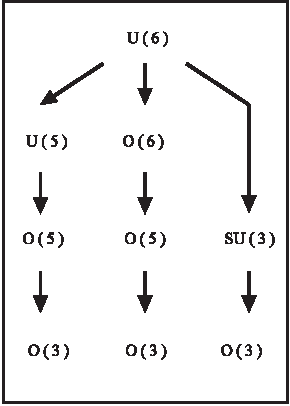
\includegraphics[scale=.65]{figure}
%
% If not, use
%\picplace{5cm}{2cm} % Give the correct figure height and width in cm
%
\caption{Please write your figure caption here}
\label{fig:A1}       % Give a unique label
\end{figure}

% For tables use
%
\begin{table}
\caption{Please write your table caption here}
\label{tab:A1}       % Give a unique label
%
% For LaTeX tables use
%
\begin{tabular}{p{2cm}p{2.4cm}p{2cm}p{4.9cm}}
\hline\noalign{\smallskip}
Classes & Subclass & Length & Action Mechanism  \\
\noalign{\smallskip}\hline\noalign{\smallskip}
Translation & mRNA$^a$  & 22 (19--25) & Translation repression, mRNA cleavage\\
Translation & mRNA cleavage & 21 & mRNA cleavage\\
Translation & mRNA  & 21--22 & mRNA cleavage\\
Translation & mRNA  & 24--26 & Histone and DNA Modification\\
\noalign{\smallskip}\hline\noalign{\smallskip}
\end{tabular}
$^a$ Table foot note (with superscript)
\end{table}
%

% %%%%%%%%%%%%%%%%%%%%%%acronym.tex%%%%%%%%%%%%%%%%%%%%%%%%%%%%%%%%%%%%%%%%%
% sample list of acronyms
%
% Use this file as a template for your own input.
%
%%%%%%%%%%%%%%%%%%%%%%%% Springer %%%%%%%%%%%%%%%%%%%%%%%%%%

\Extrachap{Glossary}



% 
\Extrachap{Solutions}

\section*{Problems of Chapter~\ref{intro}}

\begin{sol}{prob1}
The solution\index{problems}\index{solutions} is revealed here.
\end{sol}


\begin{sol}{prob2}
\textbf{Problem Heading}\\
(a) The solution of first part is revealed here.\\
(b) The solution of second part is revealed here.
\end{sol}


\printindex

%%%%%%%%%%%%%%%%%%%%%%%%%%%%%%%%%%%%%%%%%%%%%%%%%%%%%%%%%%%%%%%%%%%%%%

\end{document}





